\documentclass[12pt,twoside]{report}
\usepackage{hyperref}
\usepackage{graphicx}
\usepackage{amsmath, amssymb}
\usepackage[table]{xcolor}
\usepackage[toc,page]{appendix}
\usepackage{amssymb}
\usepackage{csquotes}
\usepackage{amsthm}
\usepackage{subdepth}
\usepackage{algorithm}
\usepackage[noend]{algpseudocode}

\theoremstyle{plain}
\newtheorem{thm}{Theorem}[chapter] % Reset theorem numbering  for each chapter

\theoremstyle{definition}
\newtheorem{defn}[thm]{Definition} % Definition numbers are dependent on theorem numbers
\newtheorem{exmp}[thm]{Example} % same for example numbers

% Ctrl + Alt + B to compile in Atom

%%%%%%%%%%%%%%%%%%%%%%%%%%%%%%%%%%%%%%%%%%%%%%%%%%%%%%%%%%%%%%%%%%%%%%%%%%%%%

% Definitions for the title page
% Edit these to provide the correct information
% e.g. \newcommand{\reportauthor}{Timothy Kimber}
\DeclareMathOperator{\E}{\mathbb{E}}

\newcommand{\reporttitle}{Symbolic Reinforcement Learning using Inductive Logic Programming}
\newcommand{\reportauthor}{Kiyohito Kunii}
\newcommand{\supervisor}{Prof. Alessandra Russo \\ Mark Law \\  Ruben L Vereecken}
\newcommand{\degreetype}{MSc in Computing Science}

%%%%%%%%%%%%%%%%%%%%%%%%%%%%%%%%%%%%%%%%%%%%%%%%%%%%%%%%%%%%%%%%%%%%%%%%%%%%%

% load some definitions and default packages
%%%%%%%%%%%%%%%%%%%%%%%%%%%%%%%%%%%%%%%%%
% University Assignment Title Page
% LaTeX Template
% Version 1.0 (27/12/12)
%
% This template has been downloaded from:
% http://www.LaTeXTemplates.com
%
% Original author:
% WikiBooks (http://en.wikibooks.org/wiki/LaTeX/Title_Creation)
%
% License:
% CC BY-NC-SA 3.0 (http://creativecommons.org/licenses/by-nc-sa/3.0/)
%
%
%%%%%%%%%%%%%%%%%%%%%%%%%%%%%%%%%%%%%%%%%
%----------------------------------------------------------------------------------------
%	PACKAGES AND OTHER DOCUMENT CONFIGURATIONS
%----------------------------------------------------------------------------------------
\usepackage[a4paper,hmargin=2.8cm,vmargin=2.0cm,includeheadfoot]{geometry}
\usepackage{textpos}
\usepackage[numbers]{natbib} % for bibliography
\usepackage{tabularx,longtable,multirow,subfigure,caption}%hangcaption
\usepackage{fncylab} %formatting of labels
\usepackage{fancyhdr} % page layout
\usepackage{url} % URLs
\usepackage[english]{babel}
\usepackage{amsmath}
\usepackage{graphicx}
\usepackage{dsfont}
\usepackage{epstopdf} % automatically replace .eps with .pdf in graphics
\usepackage{backref} % needed for citations
\usepackage{array}
\usepackage{latexsym}

% \usepackage[pdftex,pagebackref,hypertexnames=false,colorlinks]{hyperref} % provide links in pdf
\usepackage{hyperref}
\hypersetup{pdftitle={},
  pdfsubject={},
  pdfauthor={},
  pdfkeywords={},
  pdfstartview=FitH,
  pdfpagemode={UseOutlines},% None, FullScreen, UseOutlines
  bookmarksnumbered=true, bookmarksopen=true, colorlinks,
    citecolor=black,%
    filecolor=black,%
    linkcolor=black,%
    urlcolor=black}

\usepackage[all]{hypcap}


%\usepackage{color}
%\usepackage[tight,ugly]{units}
%\usepackage{float}
%\usepackage{tcolorbox}
%\usepackage[colorinlistoftodos]{todonotes}
% \usepackage{ntheorem}
% \theoremstyle{break}
% \newtheorem{lemma}{Lemma}
% \newtheorem{theorem}{Theorem}
% \newtheorem{remark}{Remark}
% \newtheorem{definition}{Definition}
% \newtheorem{proof}{Proof}


%%% Default fonts
\renewcommand*{\rmdefault}{bch}
\renewcommand*{\ttdefault}{cmtt}



%%% Default settings (page layout)
\setlength{\parindent}{0em}  % indentation of paragraph

\setlength{\headheight}{14.5pt}
\pagestyle{fancy}
\renewcommand{\chaptermark}[1]{\markboth{\chaptername\ \thechapter.\ #1}{}}

\fancyfoot[ER,OL]{\sffamily\textbf{\thepage}}%Page no. in the left on odd pages and on right on even pages
\fancyfoot[OC,EC]{\sffamily }
\renewcommand{\headrulewidth}{0.1pt}
\renewcommand{\footrulewidth}{0.1pt}
\captionsetup{margin=10pt,font=small,labelfont=bf}


%--- chapter heading

\def\@makechapterhead#1{%
  \vspace*{10\p@}%
  {\parindent \z@ \raggedright \sffamily
    \interlinepenalty\@M
    \Huge\bfseries \thechapter \space\space #1\par\nobreak
    \vskip 30\p@
  }}

%---chapter heading for \chapter*
\def\@makeschapterhead#1{%
  \vspace*{10\p@}%
  {\parindent \z@ \raggedright
    \sffamily
    \interlinepenalty\@M
    \Huge \bfseries  #1\par\nobreak
    \vskip 30\p@
  }}

\allowdisplaybreaks


% load some macros
% Here, you can define your own macros. Some examples are given below.

\newcommand{\R}[0]{\mathds{R}} % real numbers
\newcommand{\Z}[0]{\mathds{Z}} % integers
\newcommand{\N}[0]{\mathds{N}} % natural numbers
\newcommand{\C}[0]{\mathds{C}} % complex numbers
\renewcommand{\vec}[1]{{\boldsymbol{{#1}}}} % vector
\newcommand{\mat}[1]{{\boldsymbol{{#1}}}} % matrix


\date{June 2018}


% \newtheoremstyle{definition}[section]
\newtheorem{examp}{example}[section]


\begin{document}


% load title page
% Last modification: 2015-08-17 (Marc Deisenroth)
\begin{titlepage}

\newcommand{\HRule}{\rule{\linewidth}{0.5mm}} % Defines a new command for the horizontal lines, change thickness here


%----------------------------------------------------------------------------------------
%	LOGO SECTION
%----------------------------------------------------------------------------------------


\includegraphics[width = 4cm]{./figures/imperial}\\[0.5cm] 

\center % Center remainder of the page

%----------------------------------------------------------------------------------------
%	HEADING SECTIONS
%----------------------------------------------------------------------------------------

\textsc{\Large Imperial College London}\\[0.5cm] 
\textsc{\large Department of Computing}\\[0.5cm] 

%----------------------------------------------------------------------------------------
%	TITLE SECTION
%----------------------------------------------------------------------------------------

\HRule \\[0.4cm]
{ \huge \bfseries \reporttitle}\\ % Title of your document
\HRule \\[1.5cm]
 
%----------------------------------------------------------------------------------------
%	AUTHOR SECTION
%----------------------------------------------------------------------------------------

\begin{minipage}{0.4\textwidth}
\begin{flushleft} \large
\emph{Author:}\\
\reportauthor % Your name
\end{flushleft}
\end{minipage}
~
\begin{minipage}{0.4\textwidth}
\begin{flushright} \large
\emph{Supervisor:} \\
\supervisor % Supervisor's Name
\end{flushright}
\end{minipage}\\[4cm]


%----------------------------------------------------------------------------------------
%	FOOTER & DATE SECTION
%----------------------------------------------------------------------------------------
\vfill % Fill the rest of the page with whitespace
Submitted in partial fulfillment of the requirements for the MSc degree in
\degreetype~of Imperial College London\\[0.5cm]

\makeatletter
\@date 
\makeatother


\end{titlepage}


% page numbering etc.
\pagenumbering{roman}
\clearpage{\pagestyle{empty}\cleardoublepage}
\setcounter{page}{1}
\pagestyle{fancy}

%%%%%%%%%%%%%%%%%%%%%%%%%%%%%%%%%%%%
 \begin{abstract}
 Your abstract.
 \end{abstract}
%
\cleardoublepage
%%%%%%%%%%%%%%%%%%%%%%%%%%%%%%%%%%%
\section*{Acknowledgments}
% Comment this out if not needed.

\clearpage{\pagestyle{empty}\cleardoublepage}

%%%%%%%%%%%%%%%%%%%%%%%%%%%%%%%%%%%%
%--- table of contents
\fancyhead[RE,LO]{\sffamily {Table of Contents}}
\tableofcontents

% ADD BLANK PAGE
\clearpage{\pagestyle{empty}\cleardoublepage}
\pagenumbering{arabic}
\setcounter{page}{1}
\fancyhead[LE,RO]{\slshape \rightmark}
\fancyhead[LO,RE]{\slshape \leftmark}

%\fancyhead[RE,LO]{\sffamily {Table of Contents}}
\listoffigures
\listoftables
%%%%%%%%%%%%%%%%%%%%%%%%%%%%%%%%%%%%
% IMPERIAL LOGO
% \begin{figure}[tb]
% \centering
% 
\includegraphics[width = 0.4\hsize]{./figures/imperial}
% \caption{Imperial College Logo. It's nice blue, and the font is quite stylish. But you can choose a different one if you don't like it.}
% \label{fig:logo}
% \end{figure}
% Figure~\ref{fig:logo} is an example of a figure.

\chapter{Introduction}
\label{introduction}

% Including this part of chapter
There have been successful applications of deep reinforcement learning (DRL) in a number of domains, such as video games \cite{Mnih2015}, the game of Go \cite{Silver2016} and robotics \cite{Levine2015}. However, there are still a number of issues to overcome with this method.
First, it requires large dataset for training the model, and the learning is very slow and requires significant amount of computation.
Second, it is considered to be a black-box, meaning that the decision making process is unknown to the human user and therefore lacks explanation of the decision making. Third, there is no thought process to the decision making, such as understanding relational representations or planning. To tackle these problems, researchers have explored several different approaches.
One of the methods is to incorporate symbolic representations into the system \cite{Garnelo2016}. This approach is promising and shows a potential.

In this paper, we extend this symbolic representation approach and explore the potential of symbolic machine learning to solve the above issues. There are several advantages of symbolic machine learning. First of all, the decision making mechanism is understandable by humans rather than being black-box.
Second, it resembles how humans reason. Similar to reinforcement learning, there are some aspects of trial-and-error in human learning, but humans exploit reasonings to efficiently learn about their surrounding or situations. They also effectively use previous experience (e.g background knowledge) when encountering similar situations.
Finally, the recent advance of Inductive Logic Programming (ILP) research has enabled us to apply ILP in more complex situations and there are a number of new algorithms based on Answer Set Programmings (ASPs) that work well in non-monotonic scenarios.

Particularly since \cite{Garnelo2016}, there have been several researches that further explored the incorporation of symbolic reasoning into RL, but the combining of ILP and RL has not been explored. Because of the recent advancement of ILP and RL, it is natual to consider that a combination of both approaches would be the next field to explore.

In this paper, our objective is to  explore the incorporation of ILP into RL using Inductive Learning of Answer Set Programs (ILASP), which is a state-of-art ILP method that can be applied to incomplete and more complex environments.

\textcolor{red}{TODO Update this}

This background report will be part of the final report and is organised as follows: 
In Chapter \ref{background}, the background of inductive logic programming and reinforcement learning necessary for this paper are described. 
Chapter \ref{related_work} discusses previous research on relevant approach. 
Chapter \ref{project_overview} shows the tentative architecture of our new approach, using ILASP to generate a model of the environment. 
We also discuss some of the issues we currently face with the architecture and plan the implementation. 
Finally the ethics checklist is provided in Chapter \ref{ethics_checklist}.


\chapter{Background}
\label{background}

This chapter introduces necessary background of Inductive Logic Programming (Section \ref{ilp}) and Reinforcement Learning (Section \ref{rl}), which provide the foundations of our research.

\section{Inductive Logic Programming (ILP)}
\label{ilp}

\textit{Inductive Logic Programming (ILP)} is a subfield of machine learning research area aimed at the intersection between machine learning and logic programming \cite{Muggleton1991}. The purpose of ILP is to inductively derive a hypothesis H that is a solution of a learning task, which coveres all positive examples and none of negative examples, given a hypothesis language for search space and cover relation \cite{DeRaedt1997}. ILP is based on learning from entailment, as shown in Equation \ref{ilp_equation}.

\begin{equation}
B \wedge H \models E
\end{equation}
\label{ilp_equation}

where E contains all of the positive examples (E\textsuperscript{+}) and none of the negative examples (E\textsuperscript{-}).
One of the advantage of ILP over statistical machine learning is that the hypothesis that an agent learnt can be easily understood by a human, as it is expressed in first-order logic, making the learning process more transparent rather than black-box.
One of the limitations of ILP is learning efficiency and scalability. There are usually thousands or more examples in many real-world examples. Scaling ILP task to cope with large examples is a challenging task \cite{Muggleton1993}.

In this section, we briefly introduce foundation of Answer Set Programming (ASP) and inductive learning frameworks.

\subsection{Stable Model Semantics}

Having defined the syntax of clausal logic, we now introduce its semantics under the context of Stable Model. The semantics of the logic is based on the notion of interpretation, which is defined under a \textit{domain}. A domain contains all the objects that exist. In logic, it is convention to use a special interpretations called \textit{Herbrand interpretations} rather than general interpretations.

\begin{defn}
\textit{Herbrand Domain} (a.k.a \textit{Herbrand Universe}) of clause sets \textit{Th} is the set of all ground terms that are constants and function symbols appeared in \textit{Th}.
\end{defn}

\begin{defn}
\textit{Herbrand Base} of \textit{Th} is the set of all ground predicates that are formed by predicate symbols in \textit{Th} and terms in the Herbrand Domain.
\end{defn}

\begin{defn}
\textit{Herbrand Interpretation} of a set of definite clauses \textit{Th} is a subset of the Herbrand base of \textit{Th}, which is a set of ground atoms that are true in terms of interpretation.
\end{defn}

\begin{defn}
\textit{Herbrand Model} is a Herbrand interpretation if and only if a set \textit{Th} of clauses is satisfiable. In other words, the set of clauses \textit{Th} is unsatisfiable if no Herbrand model was found.
\end{defn}

\begin{defn}
\textit{Least Herbrand Model} (denoted as \textit{M(P)}) is an unique minimal Herbrand model for definite logic programs.  The Herbrand Model is a minimum Herbrand model if and only if none of its subsets is an Herbrand model.
\end{defn}
For normal logic programs, there may not be any least Herbrand Model.

%Interpretation evaluate it to true
%Interpretation evaluate it to false

\begin{examp} \normalfont (Herbrand Interpretation, Herbrand Model and M(P)) \\

P = $\begin{cases}
	p(X)  \leftarrow q(X) \\
	q (a).
      \end{cases}$
HD = \{ a \} , HB = \{ q(a), p(a) \}  \\

where HD is Herbrand Domain and HB is Herbrand Base.
Given above,  there are four Herbrand Interpretations = $\langle$ \{q(a)\}, \{p(a)\}, \{q(a), p(a)\}, \{\} $\rangle$, and one Herbrand Model (as well as M(P)) = \{q(a), p(a)\}

\end{examp}
% TODO: Use the same or similar examples for all of them.

\textit{Definite Logic Program} is a set of definite rules, and  a \textit{definite rule} is of the form \textit{h} $\leftarrow$ \textit{a}\textsubscript{1}, ..., \textit{a}\textsubscript{n}.  \textit{h} and  \textit{a}\textsubscript{1}, ..., \textit{a}\textsubscript{n} are all atoms. \textit{h} is the \textit{head} of the rule and \textit{a}\textsubscript{1}, ..., \textit{a}\textsubscript{n} are the \textit{body} of the rule.
\textit{Normal Logic Program} is a set of normal rules, and a normal rule is of the form \textit{h} $\leftarrow$ a\textsubscript{1}, ..., \textit{a}\textsubscript{n}, \textit{not b}\textsubscript{1}, ..., \textit{not  b}\textsubscript{n} where \textit{h} is the head of the rule,
 and \textit{a}\textsubscript{1}, ..., \textit{a}\textsubscript{n}, \textit{b}\textsubscript{1}, ..., \textit{b}\textsubscript{n} are the body of the rule (both the head and body are all atoms).

To solve a normal logic program \textit{Th}, the program P needs to be grounded. The \textit{grounding} of \textit{Th} is the set of all clauses that are c $\in$ \textit{Th} and variables are replaced by terms in the Herbrand Domain. 
\begin{defn}
The algorithm of grounding starts with an empty program Q = \{  \} and the relevant grounding is constructed by adding to each rule R to Q such that
\begin{itemize}
\item R is a ground instance of a rule in P.
\item Their positive body literals already occurs in the in the of rules in Q. 
\end{itemize}
The algorithm terminates when no more rules can be added to Q.

\end{defn}

\begin{examp} \normalfont Grounding \\

P = $\begin{cases}
%	p(X)  \leftarrow not \ q(X). \\
	q(X)  \leftarrow p(X). \\
	p(a).
      \end{cases}$ \\

ground(P) in this example is \{p(a), q(a)\}.

\end{examp}
\label{grounding}

%TODO Explain grounding in ASP context.
%The grounding of a normal logic program P can be obtained by replacing each rule in P with a ground instance of the rule, such that for each atom A in body\textsuperscript{+} (R) (TODO EXPLAIN WHAT THIS IS), already occurs in the head of another ground rule.
Not only the entire program needs to be grounded in order for an ASP solver to work, but also each rule must be \textit{safe}. A rule \textit{R} is safe if every variable that occurs in the head of the rule occurs at least once in body\textsuperscript{+}(R) .
Since there is no unique least Herbrand Model for a normal logic program, Stable Model of a normal logic program was defined in \cite{Gelfond1988}. In order to obtain the Stable Model of a program P, P needs to be converted using \textit{Reduct} with respect to an interpretation X. 
\begin{defn}
\begin{itemize}
The \textit{reduct} of P with respect to X can be constructed such that
\item If the body of any rule in P contains an atom which is not in X, those rules need to be removed. 
\item All default negation atoms in the remaining rules in P need to be removed.
\end{itemize}
\end{defn}

\begin{examp} \normalfont Reduct \\


P = $\begin{cases}
	p(X)  \leftarrow not\ q(X). \\
  	q (X) \leftarrow not\ p(X). \\
      \end{cases}$,  X = \{p(a), q(b)\}

Where X is a set of atoms. ground(P) is 

p(a)  $\leftarrow$ not\ q(a). \\
p(b)  $\leftarrow$ not\ q(b). \\
q(a) $\leftarrow$ not\ p(a). \\
q(b) $\leftarrow$ not\ p(b). \\

 The first step removes p(b)  $\leftarrow$ not\ q(b). and q(a) $\leftarrow$ not\ p(a).

p(a)  $\leftarrow$ not\ q(a). \\
q(b) $\leftarrow$ not\ p(b). \\

The second step removes negation atoms from the body. \\
Thus reduct P\textsuperscript{x} is (ground(P))\textsuperscript{x} =  \{p(a), q(b).\}
\end{examp}
\label{reduct}

%Any stable model is a minimal Herbrand model, and stable sets is stable models. The stable models can be found by constructing the result of the program with respect to sets of atoms X (P\textsuperscript{x} in the following 2 steps
A Stable Model of P is an interpretaiton X if and only if X is the unique least Herbrand Model of ground(P)\textsuperscript{x} in the logic program.

\subsection{Anwer Set Programming (ASP) Syntax}

\begin{defn}
Answer set of normal logic program P is a Stable Model, and Answer Set Programming (ASP) is a normal logic program with extensions: constraints, choice rules and optimisation statements. ASP program consists of a set of rules, where each rule consists of an atom and literals.
\end{defn}


A \textit{constraint} of the program P is of the form $\leftarrow$ \textit{a}\textsubscript{1}, ..., \textit{a}\textsubscript{n}, \textit{not b}\textsubscript{1}, ..., \textit{not b}\textsubscript{n}, where the rule has an empty head. The constraint filters any irrelevant answer sets. When computing ground(P)\textsubscript{x}, the empty head becomes $\perp$, which cannot be in the answer sets.
There are two types of constraints: \textit{hard constraints} and \textit{soft constraints}. Hard constraints are strictly satisfied, whereas soft constraints may not be satisfied but the sum of the violations should be minimised when solving ASP.

A \textit{choice rule} can express possible outcomes given an action choice, which is of the form
l\{h\textsubscript{1},...,h\textsubscript{m}\}u $\leftarrow$ a\textsubscript{1}, ..., a\textsubscript{n}, not b\textsubscript{1}, ..., not b\textsubscript{n} where  l and u are integers and h\textsubscript{i} for 1 $\leq$ i $\leq$ m are atoms. The head is called \textit{aggregates}.

\textit{Optimisation statement} is useful to sort the answer sets in terms of preference, which is of the form
\textit{\#minimize[a\textsubscript{1}=w\textsubscript{1},...a\textsubscript{n}=w\textsubscript{n}]} or \textit{\#maximize[a\textsubscript{1}=w\textsubscript{1},...a\textsubscript{n}=w\textsubscript{n}]} where \textit{w\textsubscript{1},..., w\textsubscript{n}} is integer weights and \textit{a\textsubscript{1},...,a\textsubscript{n}} is ground atoms.  ASP solvers compute the scores of the weighted sum of the sets of ground atoms based on the true answer sets, and find optimal answer sets which either maximise or minimise the score.

\textit{Clingo} is one of the modern ASP solvers that executes the ASP program and returns answer sets of the program (\cite{Gebser2011}), and we will use \textit{Clingo} for the implementation of this research.

%An answer set of ASP program is interpretations that make all the ruls true.
%Non-monotonicity.
%TODO ASP has true, false and unknown

\subsection{ILP under Answer Set Semantics}

There are several ILP non-monotonic learning frameworks under the answer set semantics . We first introduce two of them: \textit{Cautious Induction} and \textit{Brave Induction} (\cite{Sakama2009}), which are foundations of \textit{Learning from Answer Sets} discussed in Section \ref{section_lasp}, a state-of-art ILP framework that we will use for our research.  (for other non-monotonic ILP frameworks, see \cite{Otero2001}, \cite{Inoue2014}, \cite{Corapi2012} and \cite{DeRaedt1997}).
\subsubsection{Cautious Induction }
% Sakama 2008 has no concept of negative examples in this paper.
Cautious Induction task \footnote{This is more general definition of Cautious Induction than the one defined in \cite{Sakama2009}, as the concept of negative examples was not included in the original definition.} is of the form $\langle$ B, E\textsuperscript{+}, E\textsuperscript{-} $\rangle$, where B is the background knowledge, E\textsuperscript{+} is a set of positive examples and E\textsuperscript{-} is a set of negative examples.

 H $\in$ ILP\textsubscript{cautious} $\langle$ B, E\textsuperscript{+}, E\textsuperscript{-} $\rangle$ if and only if  there is at least one answer set A of B $\cup$ H (B $\cup$ H is satisfiable) such that for every answer set A of B $\cup$ H: \\
\begin{enumerate}
\item $\forall$ e $\in$ E\textsuperscript{+} : e $\in$ A
\item $\forall$ e $\in$ E\textsuperscript{-} : e $\notin$ A
\end{enumerate}

\begin{examp} \normalfont Cautious Induction \\

B = $\begin{cases}
	exercises  \leftarrow not \ eat\_out. \\
	eat\_out \leftarrow exercises. \\
      \end{cases}$
E\textsuperscript{+} = \{tennis\},      E\textsuperscript{-} = \{eat\_out \} \\

One possible  H $\in$ ILP\textsubscript{cautious} is \{tennis$ \leftarrow$ exercises, $\leftarrow$ not tennis \}.
\end{examp}
\label{cautious_induction_example}

The limitation of Cautious Induction is that positive examples must be true for all answer sets and negative examples must not be included in any of the answer sets. These conditions may be too strict in some cases, and Cautious Induction is not able to accept a case where positive examples are true in some of the answer sets but not all answer sets of the program.

\begin{examp} \normalfont Limitation of Cautious Induction \\

B = $\begin{cases}
	1\{situation(P, awake), situation(P, sleep)\}1 \leftarrow person(P). \\
	person(john).
      \end{cases}$ \\

Neither of \textit{situation(john, awake)} nor \textit{situation(john, sleep)} is false in all answer sets. In this example, it only returns person(john). Thus no examples could be given to learn the choice rule.
\end{examp}

\label{limitation_cautious}

\subsubsection{Brave Induction}
Brave Induction task is of the form $\langle$ B, E\textsuperscript{+}, E\textsuperscript{-} $\rangle$ where, B is the background knowledge, E\textsuperscript{+} is a set of positive examples and E\textsuperscript{-} is a set of negative examples.
 H $\in$ ILP\textsubscript{brave} $\langle$ B, E\textsuperscript{+}, E\textsuperscript{-} $\rangle$ if and only if there is at least one answer set A of B $\cup$ H such that: \\
\begin{enumerate}
\item $\forall$ e $\in$ E\textsuperscript{+} : e $\in$ A \\
\item $\forall$ e $\in$ E\textsuperscript{-} : e $\notin$ A \\
\end{enumerate}

\begin{examp} \normalfont Brave Induction \\

B = $\begin{cases}
	exercises  \leftarrow not \ eat\_out. \\
	tennis \leftarrow holiday \\
      \end{cases}$
E\textsuperscript{+} = \{tennis\},   E\textsuperscript{-} = \{eat\_out \} \\

One possible  H $\in$ ILP\textsubscript{brave} is \{tennis\}, which returns \{tennis, holidy, exercises\} as answer sets.
\end{examp}
\label{brave_induction_example}

The limitation of Brave Induction that it cannot learn constraints, since the above conditions for the examples only apply to at least one answer set A, whereas constrains rules out all answer sets that meet  the conditions of the Brave Induction.

\begin{examp} \normalfont Limitation of Brave Induction (Example) \\

B = $\begin{cases}
	1\{situation(P, awake), situation(P, sleep)\}1 \leftarrow person(P). \\
	person(C) \leftarrow super\_person(C). \\
	super\_person(john).
	\end{cases}$ \\

In order to learn the  constraint hypothesis H = \{ $\leftarrow$ not situation(P, awake), super\_person(P)\}, it is not possible to find an optimal solution.
\end{examp}
\label{limitation_brave}

\subsection{Inductive Learning of Answer Set Programs (ILASP)}
\label{section_lasp}

\subsubsection{Learning from Answer Sets (LAS)}
\textit{Learning from Answer Sets (LAS)} was developed in \cite{Law2014} to faciliate more complex learning tasks that neither Cautious Induction nor Brave Induction could learn.
Examples used in LAS are \textit{Partial Interpretations}, which are of the form $\langle$ e\textsuperscript{inc}, e\textsuperscript{exc}$\rangle$. (called \textit{inclusions} and \textit{exclusions} of \textit{e} respectively).  A Herbrand Interpretation extends a partial interpretation if it includes all of e\textsuperscript{inc} and none of e\textsuperscript{exc}.
LAS is of the form $\langle$ B, S\textsubscript{M}, E\textsuperscript{+}, E\textsuperscript{-} $\rangle$, where B is background knowledge, S\textsubscript{M} is hypothesis space, and E\textsuperscript{+} and E\textsuperscript{-} are examples of positive and negative partial interpretations. S\textsubscript{M} consists of a set of normal rules, choice rules and constraints. S\textsubscript{M} is specified by \textit{language bias} of the learning task using \textit{mode declaration}. Mode declaration specifies what can occur in a hypothesis by specifying the predicates, and consists of two parts: \textit{modeh} and \textit{modeb}.  \textit{modeh} and \textit{modeb} are the predicates that can occur in the head of the rule and body of the rule respectively. Language bias is the specification of the language in the hypothesis in order to reduce the search space for the hypothesis.

\begin{defn}{Learning from Answer Sets (LAS)}

Given a learning task T, the set of all possible inductive solutions of T is denoted as ILP\textsubscript{LAS}(T), and a hypothesis H is an inductive solution of ILP\textsubscript{LAS}(T) $\langle$ B, S\textsubscript{M}, E\textsuperscript{+}, E\textsuperscript{-} $\rangle$ such that:
\begin{enumerate}
\item H $\subseteq$ S\textsubscript{M}
\item $\forall$ e $\in$ E\textsuperscript{+} : $\exists$ A $\in$ Answer Sets(B $\cup$ H) such that A extends e
\item $\forall$ e $\in$ E\textsuperscript{-} : $\nexists$ A $\in$ Answer Sets(B $\cup$ H) such that A extends e
\end{enumerate}

\end{defn}


%S\textsubscript{M} consists of all rules given the language bias.

%\begin{examp} \normalfont LAS
%
%TODO
%%B = $\begin{cases}
%%	exercises  \leftarrow not \ eat\_out. \\
%%	tennis \leftarrow holiday \\
%%      \end{cases}$ \\
%%E\textsubscript{+} = tennis \\
%%E\textsubscript{-} = eat\_out \\
%
%\end{examp}
%\label{las_example}

% Limitation of LAS??

\subsubsection{Inductive Learning of Answer Set Programs (ILASP)}

\textit{Inductive Learning of Answer Set Programs (ILASP)} is an algorithm that is capable of solving LAS tasks, and is based on two fundamental concepts: \textit{positive solutions} and \textit{violating solutions}.

A hypothesis H is a positive solution if and only if
\begin{enumerate}
\item H $\subseteq$ S\textsubscript{M}
\item $\forall$ e\textsuperscript{+} $\in$ $\exists$ A $\in$ Answer Sets(B $\cup$ H) such that A extends e\textsuperscript{+}
\end{enumerate}
A hypothesis H is a violating solution if and only if
\begin{enumerate}
\item H $\subseteq$ S\textsubscript{M}
\item $\forall$ e\textsuperscript{+} $\in$ E\textsuperscript{+} $\exists$ A $\in$ Answer Sets(B $\cup$ H) such that A extends e\textsuperscript{+}
\item $\exists$ e\textsuperscript{-} $\in$ E\textsuperscript{-} $\exists$ A $\in$ Answer Sets(B $\cup$ H) such that A extends e\textsuperscript{-}\\
\end{enumerate}

Given both definitions of positive and violating solutions, ILP\textsubscript{LAS} $\langle$ B, S\textsubscript{M}, E\textsuperscript{+}, E\textsuperscript{-} $\rangle$is positive solutions that are not violating solutions.

\subsubsection{A Context-dependent Learning from Answer Sets }
\textit{Context-dependent learning from ordered answer sets ($ILP_{LOAS}^{context}$)} is a further generalisation of ILP\textsubscript{LOAS} with \textit{context-dependent examples} \cite{Law2016}
Context-dependent examples are examples that each unique background knowledge (context) only applies to specific examples. This way the background knowledge is more structured rather than one fixed background knowledge that are applied to all examples.
Formally, partial interpretation is of the form $\langle$ e, C $\rangle$ (called \textit{context-dependent partial interpretation (CDPI)}), where \textit{e} is a partial interpretation and C is called \textit{context}, or an ASP program without weak constraints.
A \textit{context-dependent ordering example (CDOE)} is of the form $\langle$ $\langle$e\textsubscript{1}, C\textsubscript{1} $\rangle$, $\langle$ e\textsubscript{2}, C\textsubscript{2} $\rangle$$\rangle$, which is a pair of CDPI. An APS program P \textit{bravely respects o} if and only if
\begin{enumerate}
 \item $\exists$ $\langle$ A\textsubscript{1}, A\textsubscript{2} $\rangle$ such that A\textsubscript{1} $\in$ Answer Sets(P $\cup$ C\textsubscript{1}),  A\textsubscript{2}, $\in$ Answer Sets(P $\cup$ C\textsubscript{2}), A\textsubscript{1} extends e\textsubscript{1}, A\textsubscript{2} extends e\textsubscript{2} and A\textsubscript{1} $\prec$\textsubscript{P} A\textsubscript{2}
\end{enumerate}

 Similarly, an APS program P \textit{cautiously} respects \textit{o} if and only if
\begin{enumerate}
 \item $\forall$ $\langle$ A\textsubscript{1}, A\textsubscript{2} $\rangle$ such that A\textsubscript{1} $\in$ Answer Sets(P $\cup$ C\textsubscript{1}),  A\textsubscript{2}, $\in$ Answer Sets(P $\cup$ C\textsubscript{2}), A\textsubscript{1} extends e\textsubscript{1}, A\textsubscript{2} extends e\textsubscript{2} and A\textsubscript{1} $\prec$\textsubscript{P} A\textsubscript{2}
\end{enumerate}

$ILP_{LOAS}^{context}$ task is of the form T = $\langle$ B, S\textsubscript{M}, E\textsubscript{+}, E\textsubscript{-}, O\textsuperscript{b},O\textsuperscript{c}$\rangle$ where O\textsuperscript{b} and O\textsuperscript{c} are brave and cautious orderings respectively, which are sets of ordering examples over set of positive partial interpretations E\textsuperscript{+}.
A hypothesis H is an inductive solution of T if and only if
\begin{enumerate}
\item H $\subseteq$ S\textsubscript{M} in $ILP_{LOAS}^{context}$
\item $\forall$$\langle$ e, C$\rangle$ $\in$ E\textsuperscript{+}, $\exists$A $\exists$ A $\in$ Answer Sets (B $\cup$ C $\cup$ H) such that A extends e
\item $\forall$$\langle$ e, C$\rangle$ $\in$ E\textsuperscript{-}, $\nexists$A $\exists$ A $\in$ Answer Sets (B $\cup$ C $\cup$ H) such that A extends e
%\item $\forall$o $\in$ O\textsuperscript{b} B $\cup$ H bravely respects o
%\item $\forall$o $\in$ O\textsuperscript{c} B $\cup$ H cautiously respects o
\end{enumerate}

The two main advantages of adding contex-dependent are that it increases the efficiency of learning tasks, and more expressive structure of the background knowlege to particular examples. These features will be useful when a game agent is in two different environmets as discussed in Section \ref{model_generation_and_update}.

\section{Reinforcement Learning (RL)}
\label{rl}
\textit{Reinforcement learning (RL)} is a subfield of machine learning regarding how an agent behaves in an environment in order to maximise its total reward. As shown in Figure \ref{agent_env}, the agent interacts with an environment, and at each time step the agent takes an action and receives observation, which affects the environment state and the reward (or penalty) it receives as the action outcome. In this section, we briefly introduce the background in RL necessary for our research.

\begin{figure}[!htb]
\centering
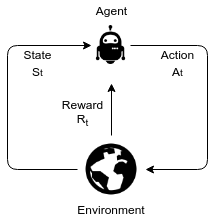
\includegraphics[width=6cm, height=6cm]{./figures/agent_env}
\caption{Agent and Environment}
\label{agent_env}
\end{figure}

\subsection{Markov Decision Process (MDP)}
\label{mdp_subsection}
An agent interacts with an environment at a sequence of discrete time step, which is part of the sequential history of observations, actions and rewards. The sequential history is formalised as H\textsubscript{t} = O\textsubscript{1}, R\textsubscript{1}, A\textsubscript{1}, ..., A\textsubscript{t-1}, O\textsubscript{t}, R\textsubscript{t}.  A \textit{state} is a function of the history S\textsubscript{t} = f(H\textsubscript{t}), which determines the next environment.  A state S\textsubscript{t} is said to have \textit{Markov property} if and only if P[S\textsubscript{t+1} $\vert$ S\textsubscript{t}] = P[S\textsubscript{t+1} $\vert$ S\textsubscript{1}, ..., S\textsubscript{t}]. In other words, the probability of reaching S\textsubscript{t+1} depends only on S\textsubscript{t}, which captures all the relevant information from the earilier history (\cite{Puterman1994}).
When an agent must make a sequence of decision, the sequential decision problem can be formalised using \textit{Markov decision process (MDP)}. MDP formaly represents a fully observable environment of an agent for RL.

A MDP is of the form $\langle$ S, A, T\textsubscript{a}, R\textsubscript{a}, $\gamma$ $\rangle$ where:

\begin{itemize}
\item S is the set of finite states that is observable in the environment.
\item A is the set of finite actions taken by the agent.
\item T\textsubscript{a}(s, s$^\prime$) is a state transition in the form of probability matrix Pr(S\textsubscript{t+1} = s$^\prime$ $\vert$ s\textsubscript{t} = s, a\textsubscript{t} = a), which is the probablity that action \textit{a} in state \textit{s} at time \textit{t} will result in state \textit{s$^\prime$} at time \textit{t+1}.
\item R is a reward function R\textsubscript{a}(s, s$^\prime$) = $\displaystyle \E[R\textsubscript{t+1} $ $\vert$ S\textsubscript{t} = s, A\textsubscript{t} = a], the expected immediate reward that action \textit{a} in state \textit{s} at time \textit{t} will return.
\item $\gamma$ is a discount factor $\gamma$ $\in$ [0,1], which represents the preference of the agent for the present reward over future rewards.
\end{itemize}

%$\displaystyle \E[R\textsubscript{t+1} \vert$ S\textsubscript{t} = s]
\subsection{Policies and Value Functions}
\label{policy_value_functions_subsection}

\textit{Value functions} estimate the expected return, or expected future rewarded,  for a given action in a given state. The expected reward for an agent is dependent on the agent's action.  The state value function v\textsubscript{$\pi$}(s) of an MDP under a policy $\pi$ is the expected return starting from state \textit{s}, which is of the form:

\begin{equation}
v\textsubscript{$\pi$}(s) = \displaystyle \E [G\textsubscript{t} \vert S\textsubscript{t} = s]
\end{equation}

where G\textsubscript{t} = R\textsubscript{t+1} + $\gamma$R\textsubscript{t+2} + ... $\gamma$\textsuperscript{T-1}R\textsubscript{T} , or the total discounted reward from \textit{t}.

The optimal state-value function v\textsuperscript{*}(s) maximises the value function over all policies in the MDP, which is of the form:

\begin{equation}
v\textsuperscript{*}(s) = \underset{\pi}{\max} \ v\textsubscript{$\pi$}(s)
\end{equation}

The optimal action-value function q\textsuperscript{*}(s) maximises the action-value function over all policies in the MDP, which is of the form:

\begin{equation}
q\textsuperscript{*}(s, a) = \underset{\pi}{\max} \ q\textsubscript{$\pi$}(s, a)
\end{equation}

A solution to the sequential decision problem is called a \textit{policy $\pi$}, a sequence of actions that leads to a solution. An optimal policy achieves the optimal value function (or action-value function), and it can be computed by maximising over the optimal value function (or action-value function).

\textcolor{red}{TODO BELLMAN OPTIMALITY EQUATION}
%A policy $\pi$ is optimal if it maximises the action-value function q()
%The transition and reward functions are not necessary to be known to compute $\pi$.
%Among all possible value functions, an \textit{optimal policy $\pi^*$} is the one that maximise the total rewards in the environment.
%The optimal policy $\pi$\textsuperscript{*} corresponds to v\textsuperscript{*}(s)

%\begin{equation}
%\pi \textsuperscript{*} =
%%\pi \textsuperscript{*} = arg max v\textsubscript{\pi}(s)
%\end{equation}

%Reinforcement learning is a method to get approximated optimal solution.
%TODO on-policy and off-policy learning.

%A\textsubscript{t} = $\pi$(S\textsubscript{t})
%
%One of the common possibilities is that the agent chooses an action in order to maximise the discounted sum of future rewards.
%
%A\textsubscript{t} to maximise R\textsubscript{t+1} + $\gamma$ R\textsubscript{t+2} + $\gamma^2$ R\textsubscript{t+3} + ...
%
%An action-value function evaluate a particular state by taking an action according the policy
%
%q\textsubscript{$\pi$} = $\displaystyle \E[R\textsubscript{t+1} $[R\textsubscript{t+1} + $\gamma$ R\textsubscript{t+2} + $\gamma^2$ R\textsubscript{t+3} + ... $\vert$ S\textsubscript{t} = s, A\textsubscript{t} = a, A\textsubscript{t+1 } = a,]

\textcolor{red}{TODO Value iterations}

\subsection{Model-based and Model-free Reinforcement Learning}
\label{model_base_model_free_subsection}

\textcolor{red}{TODO delte dyna and focus more on model-based approach}

A model M is a representation of an environment that an agent can used to understand how the environment should look like . Model-based learning is that the agent learns the model and plan a solution using the learnt model. Once the agent learns the model, the problem to be solved becomes a planning problem for a series of actions to achieve the agent's goal.
Most of the reinforcement learning problems are model-free learning, where M is unknown and the agent learns to achieve the goal by solely interacting with the environment. Thus the agent knows only possible states and actions, and the transition state and reward probability functions are unknown.

The performance of model-based RL is limited to optimal policy given the model M. In other words, when the model is not a representation of the true MDP, the planning algorithms will not lead to the optimal policy, but a suboptimal policy.

One algorithm which combine both aspects of model-based and model-free learning to solve the issue of sub-optimality is called Dyna (\cite{Sutton1990}), which is shown in Figure \ref{dyna}.

\begin{figure}[!htb]
\centering
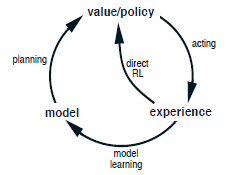
\includegraphics[width=8cm, height=6cm]{./figures/dyna}
%\caption{Relationships among learning, planning and acting \cite{Montague1999}}
\caption{Relationships among learning, planning and acting}
\label{dyna}
\end{figure}

Dyna learns a model from real experience and use the model to generate simulated experience to update the evaluation functions.
This approach is more effective because the simulated experience is relatively easy to generate compared building up real experience, thus less iterations are required.

\subsection{Temporal-Difference (TD) Learning}
\label{td_learning_section}

To solve a MDP, one of the approaches is called \textit{Temporal-Difference (TD) Learning}.
TD is an online model-free learning and learns directly from episodes of imcomplete experiences without a model of the environment.
TD updates the estimate by using the estimates of value function by bootstrap, which is formalised as

\begin{equation}
\centering
V(S\textsubscript{t}) \leftarrow V(S\textsubscript{t}) + \alpha[R\textsubscript{t+1} + \gamma V(S\textsubscript{t+1}) - V(S\textsubscript{t})]
\end{equation}

where R\textsubscript{t+1} + $\gamma$ V(S\textsubscript{t+1}) is the target for TD update, which is biased estimated of v\textsubscript{$\pi$} (S\textsubscript{t}), and $\delta$ = R\textsubscript{t+1} + $\gamma$ V(S\textsubscript{t+1}) - V(S\textsubscript{t}) is called TD error, which is the error in V(S\textsubscript{t}) available at time t+1.
Since TD methods only needs to know the estimate of one step ahead and does not need the final outcome of the episodes, it can learn online after every time step. TD also works without the terminal state, which is the goal for an agent.
TD(0) is proved to converge to v\textsubscript{$\pi$} in the table-based case (non-function approximation).
However, because bootstraping updates an estimate for an estimate, some bias are inevitable.
%In addition, TD method is sensitive to initial value, (but low variance).

%\begin{equation}
%\textbf{	V(S\textsubscript{t} \leftarrow V(S\textsubscript{t} + \alpha (R\textsubscript{t+1} + \gamma V(S\textsubscript{t+1}) - V(S\textsubscript{t}))
%}\end{equation}

\textit{Q-learning} is off-policy TD learning defined in \cite{Watkins}, where the agent only knows about the possible states and actionns. The transition states and reward probability functions are unknown to the agent.
It is of the form:

\begin{equation}
Q(s\textsubscript{t},a\textsubscript{t}) \leftarrow Q(s\textsubscript{t},a\textsubscript{t}) +  \alpha(R\textsubscript{t+1} + \gamma  max (a+t) Q(s\textsubscript{t+1}, a\textsubscript{t+1}) - Q(s\textsubscript{t}, a\textsubscript{t}))
\end{equation}

where $\alpha$ is the learning rate, $\gamma$ is a discount rate between 0 and 1. The equation is used to update the state-action value function called Q function. The function Q(S,A) predicts the best action A in state S to maximise the total cumulative rewards.

\begin{algorithm}
\caption{Q-learning (off-policy TD control)}\label{euclid}
\begin{algorithmic}[1]
\Procedure{ILASP(RL) (B and E)}{}

\State $\text{Initialise Q(s,a) arbitrarily}$
\State $\text{Repeat (for each episode)}$
\State $\text{Choose a from s using policy derived from Q (e.g, epsilon-greedy)}$
\State $\text{Take action a, observe r,  s$\prime$}$


%\begin{equation}
%Q(s,a) \leftarrow Q(s,a) +  \alpha(R\textsubscript{t+1} + \gamma  max (a+t) Q(s$\prime$, a$\prime$) - Q(s\textsubscript{t}, a\textsubscript{t}))
%s \gets s$\prime$
%\end{equation}

%    \State $\textit{H (inductive solutions)} \gets \text{run ILASP(T)}$
%    \State $\textit{plan(actions, states) answer sets} \gets \text{AS(B, H)}$
%    \While {actions in P}
%        \State $\textit{observed state} \gets \text{run clingo(T)}$
%        \If {$ \textit{observed state} \neq \textit{predicted state} $}
%            \State $\textit{H} \gets \text{run ILASP(T)}$
%            \EndIf
        % \If {$ \textit{observed state not equal \textit{predicted state $} 
        % \EndIf
%    \EndWhile
    % \If {$ new \ background \ encountered $}
    %     % \State $\textit{H} \gets \text{run ILASP(T)}$
    % \EndIf
    % \For{i from 0 to N} 
    %     \If {$ A[i]\ is \ in \ T$}
    %         \State \Return $FALSE$
    %     \Else 
    %         \State Add A[i] to T   
    %     \EndIf
    % \EndFor
% \State \Return $TRUE$
%\EndWhile

\EndProcedure
\caption{XXXX }
\end{algorithmic}
\end{algorithm}

\begin{equation}
Q(s\textsubscript{t},a\textsubscript{t}) = E [R\textsubscript{t+1} + \gamma R\textsubscript{t+2} + \gamma^2 R\textsubscript{t+3} + ... \vert s\textsubscript{t},a\textsubscript{t} ]
\end{equation}


Q-learning is guaranteed to converge to a optimal policy in a fininte tabulara representation.
\textcolor{red}{Paper Jaakkola et al. 1993}

The optimal Q-function Q\textsuperscript{*}(s,a) is directly approximated by the learned action-value function Q.

% Model free can be done using Monte Carlo Policy evaluation
% One way to solve the Bellman Optimality equation is Q-leraning
% U(s) = max a Q(s,a)
% The function is estimated by Q-learning, which repeately updates Q(s,a) using the Bellman Equation.
Q-learning learns the value of its deterministic greedy policy from the experience and gradually converge to the optimal Q-function. It also explored following \textit{$\epsilon$-greedy policy}, which is a stochastic greedy policy, but with the probability of $\epsilon$, the agent chooses an action randomly instea of the greedy action.

\subsection{Function Approximation}
\label{function_approximation}
Q-learning with tarbular method works when every state has Q(s,a). In case of very large MDPs, however, 
it may not be possible to represent all states with a lookup table.
For example,  robot arms has a continuous states in 3D dimentional space. 

These problems motivate the use of function approximation, which estimates value function with function approximation.  Not only it is  represented in tabular form, but also in the form of a parameterized function with weight vector w $\in \R\textsuperscript{d}$ where $\R\textsuperscript{d}$ is XXX

Unlike Q-table, changing one weight updates the estimated value of not only one state, but many states, and this generalisation makes it more flexible to apply different scenarios that tabular approach could not be applied. 

The reason we are introduing this function approximation is not because we will use it in our new algorithm, but for the benchmark that we compare our algorithm with. 

\subsubsection{The Prediction Objective ($\overline{VE}$)}
With function approximation, an update at one state changes many other states, and therefore the values of all states will not be exactly accurate, and there is a tradeoff among states as to which state we make it more accurate, while other might be  less accurate. 

The error in a state s is the squeare of the difference between the approximate value $\hat{v}$(s,w) and the true value v\textsubscript{$\pi$}(s). The objective function can be defined by weighting it over the statespace by $\mu$, the \textit{Mean Squared Value Error}, denoted $\overline{VE}$.

\begin{equation}
\overline{VE}(w) \doteq \sum_{s \in S} \mu (s) \big[ v\textsubscript{$\pi$}(s) - \hat{v}(s,w) \big]\textsuperscript{2}.
\end{equation}
\label{ve}

\subsubsection{Stochastic gradient descent (SGD)}
Stochastic gradient descent methods are commonly used to learn function approximation in value prediction, which works well for online reinforcement learning.
TODO EXPLAIN ONLINE VS OFFLINE LEARNING

\begin{equation}
 w \doteq  \begin{pmatrix}  w\textsubscript{1}  \\ w\textsubscript{2} \\ \vdots \\ w\textsubscript{n}   \end{pmatrix}
\end{equation}

and $\hat{v}$(s,w) is a differentiable function of w for all s $\in$ S. 

minimize the $\overline{VE}$ on the observed examples. \textit{Stochastic gradient-descent (SGD) } adjusts the weights vector by a fraction of alpha in the direction what will reduce the error on that example the most. Formally, it is defined as 

\begin{equation}
\begin{split}
w\textsubscript{t+1} & \doteq w\textsubscript{t} -  \frac{1}{2} \alpha  \bigtriangledown \big[ v\textsubscript{$\pi$}(S\textsubscript{t}) - \hat{v}(S\textsubscript{t}, w\textsubscript{t}) \big]\textsuperscript{2}. \\
& = w\textsubscript{t} -  \alpha  \big[ v\textsubscript{$\pi$}(S\textsubscript{t}) - \hat{v}(S\textsubscript{t}, w\textsubscript{t}) \big] \bigtriangledown \hat{v}(S\textsubscript{t}, w\textsubscript{t}).
\end{split}
\end{equation}

where $\alpha$ is step-size, 

The dradient of J(w) is defined as 

\begin{equation}
\bigtriangledown\textsubscript{w} J(w) =  \begin{pmatrix} \frac{\partial J(w)}{\partial w\textsubscript{1}}  \\ \vdots \\ \frac{\partial J(w)}{\partial w\textsubscript{n}}   \end{pmatrix}
\end{equation}

\begin{equation}
w\textsubscript{t+1} \doteq w\textsubscript{t} + \alpha \big[ U\textsubscript{t} - \hat{v}(S\textsubscript{t}, w\textsubscript{t})\big] x(S\textsubscript{t})
\end{equation}

\subsubsection{Linear Value Function Approximation}

Formally,
\begin{equation}
\hat{q}(s,a) \approx q\textsubscript{$\pi$} (s,a)
\end{equation}

Represent state by a \textit{feature vector}

\begin{equation}
x(S) = \begin{pmatrix} x\textsubscript{1}(S) \\ \vdots \\ x\textsubscript{n}(S)  \end{pmatrix}
\end{equation}

Use SGD updates with linear function approximation. The gradient of the approximate value function with respect to w is 

\textcolor{red}{Add proof here}

\begin{equation}
\bigtriangledown \hat{v}(s,w) = x(s)
\end{equation}

Thus the general SGD update defined in XX can be simplified to 

Represent value function by a linear combination of features

\begin{equation}
\hat{v}(S,w) = x(S)\textsuperscript{T}w = \sum_{j=1}^{n} x\textsubscript{j} (S) w\textsubscript{j}
\end{equation}

Objective function is 
The error in a state s is the square of the difference between the approximate value 
$\hat{v}$(S,w) and the true value v(S,w). 
\begin{equation}
J(w) = \displaystyle \E \textsubscript{$\pi$} \big[ (v\textsubscript{$\pi$}(S) -  \hat{v}(S,w))\textsuperscript{2} \big]
\end{equation}

Linear TD(0) is guaranteed to converge to clobal optimum

One disadvantage of the linear method is that it cannot express any relationship between features. For example, it cannot represent that feature \textit{i} is useful only if feature \textit{j} is not present. 

Nevertheless,  this approach is sufficient enough for our experiment, which will be described in Chapter XXX.

There are different linear methods to represents states as features, such as polynomials, fourier basis, or radial basis functions to name a few. Feature construction depends on a problem you are solving. In the next section, we introduce \textit{Tile Coding} which will be used for our benchmark. 

\subsubsection{Tile Coding \textcolor{red}{TODO REFERENCE OF THIS METHOD}}

State set is represented as a continuous two-dimentionala space. If a state is within the space, then the value of the  corrensponding feature is set to be 1 to indicate that the feature is present, while 0 indicates that the feature is absent. This way of representing the feature is called \textit{binary feature}.  \textit{Coarse coding} represents a state with which binary features are present within the space. 
One area is associated with one weight w, and training at a state will affect the weight of all the areas overlapping that state. the approximate value function will be updated within at all states within the union of the areas, and a point that has more overlap will be more affected, as illustrated in Figure XX.

The size and shape of the areas will determine the degree of the generalisation. Large areaas will have more generalisation
the change of the weight in that state will affect all other states within the intersection of the spaces. 

The degree of overlap within a space will determined the degree of the generalisation. 

The shape of the space also affect how it is generalised. 

\begin{figure}[!htb]
\centering
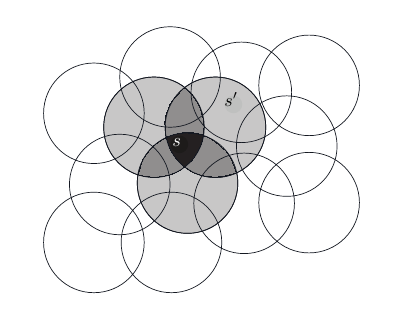
\includegraphics[width=8cm, height=6cm]{./figures/coarse_coding}
%\caption{Relationships among learning, planning and acting \cite{Montague1999}}
\caption{Relationships among learning, planning and acting \textcolor{red}{Update this figure}}
\label{dyna}
\end{figure}

\textit{Tile coding} is a type of coarse coding. \textit{Tiling} is a partition of state space, and each element of the partition is called a \textit{tile}. 

In order to do coarse coding with tile coding, multiple tilings are required, each tiling is offset from one another by a fraction of a tile width. 

As illustrated in Figure XXX, when a state occurs, several features with corresponding tiles become active, 

\begin{figure}[!htb]
\centering
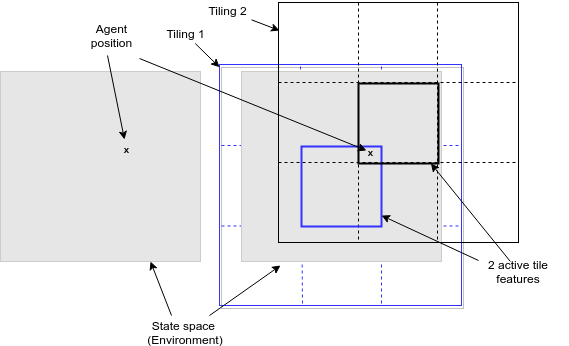
\includegraphics[width=1.0\textwidth]{./figures/tile_coding}
%\caption{Relationships among learning, planning and acting \cite{Montague1999}}
\caption{Relationships among learning, planning and acting \textcolor{red}{Update this figure}}
\label{dyna}
\end{figure}

Tile coding has computational advantage, since each component of tiling is binary value,  XXXX.

a trained state will be generalised to other states if they are within any of the same tiles. 

Similar to coarse coding, the size and shape of tiles will determine the degree of approximation. 

\subsection{Transfer Learning}
\label{transfer_learning}

Transfer learning is a method that knowledge learnt in one or more tasks can be used to learn a new task better than if without the knowlege in the first task. 

Transfer learning is an active research areas in machine learning, but not many have been done in RL. 
Since training tend to be time consuming and computational expensive, transfer learning allow the trained model to be applied in a different setting. 

Transfer learning in RL is particularly important since most of the RL research have been done in a simulation or game scenarios, and training RL models in a real physical environment is more expensive to conduct. 

Even in a virtual environments like games,  the transfer learning between different tasks will greatly will have a big impact on potential applications. 

This will also speed up learning 

Transfer learning in ILP domain have been proved to be successful in many fields, 

Since this project is combining ILP into RL senarios, this has a potential for extending this particular research. 

We conducted experiements on transfer learning capabilities, which we describe in XXX. 

One of the  purposes of transfer learning is so that the agent requires less time to learn a new task with the help of what was learn in previous tasks.  


Another goal would be to measure how effectively the agent reuses its knoledge in a new task. 
In this case the performan of learningon the first task is usally not measured. 

There are many different matrices used to measure the performance of the transfer learning.
Five common matrics are defined in XX as follow.


TODO source task selection

%Compare with human play, which is used in DeepMind Atari paper. 


\begin{itemize}
\item Jumpstart
\item Asymptotic Performance
\end{itemize}

Since each matric measures different aspect of transfer learning, using multiple metrics would provide more comprehensive views of the performance of an RL algorithm.

\begin{equation}
\begin{split}
r = \frac{Area under curve with transfer - area under curve without transfer}{area under curve without transfer}
\end{split}
\end{equation}
REFERENCE


\chapter{Framework}
\label{framework}
% \section{Learning Pipeline}
% \label{learning_pipeline_section}

The overall pipeline is shown in Figure \ref{fig:pipeline}. By interacting with the environment, an agent accumulates state transition experiences as positive examples, which is used by ILASP to learn and improve hypothesis.
The agent also records surrounding information it has seen as background knowledge, which is used to make a plan together with the hypothesis that ILASP learns by solving an answer set program. 
Mechanisms of each step is explain in details in the following sections. 

\begin{figure}[!htb]
\centering
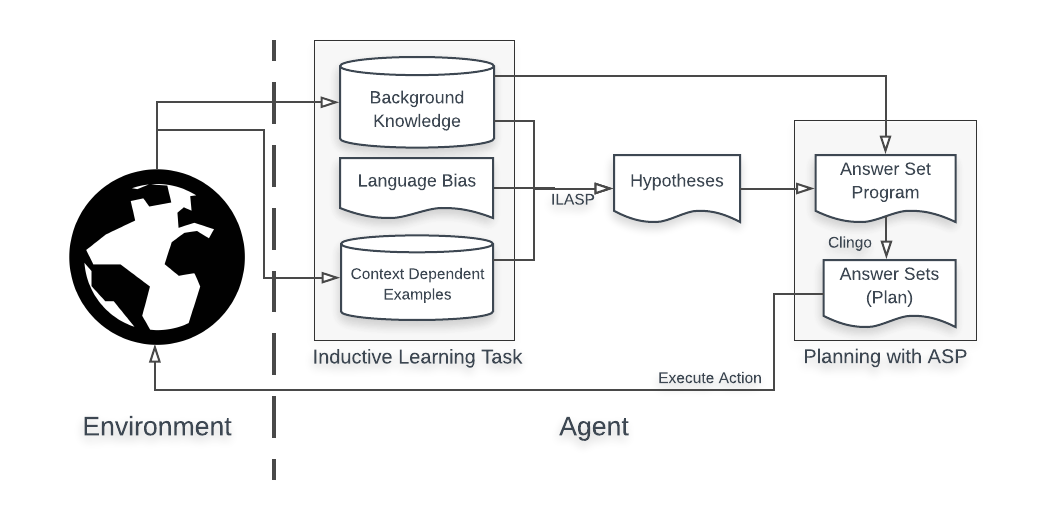
\includegraphics[width=0.8\textwidth]{./figures/architecture}
\caption{Reinforcement learning pipeline using ILASP. ILASP learns to generate a modelof the environment, or hypothesis, and updates it based on the interaction with the environment. }
\label{fig:pipeline}
\end{figure}

\section{Experience Accumulation}
\label{experience_accumulation}
\textcolor{red}{Draw an illustration of the difference between exploration and las part}\\
\textcolor{red}{Related these with Definition of ILASP}\\
The first step is to accumulate experience by interacting with the environment. Similar to tranditional RL agent, an agent explores an environment randomly until it reaches the goal once. 
Every time the agent takes an action during the exploration phase, these experiences need to be recorded in two different forms: \textit{state transition experience} and \textit{environment experience}.

\subsection{State transition experience}
\textit{State transition experience} contain information about how the state transition at each time step.
 It is the same as E\textsuperscript{+} in ILASP, especially positive examples for ILASP in ASP syntax, which is of the form:

\begin{equation}
\begin{split}
\textsf{\#pos(} & \textsf{\{state\_after((X2,Y2))\}},\\
& \{\textsf{all other state\_after that did not happen}\}, \\
& \{\textsf{state\_before((X1,Y1)). action(A). surrounding information}\}).
\end{split}
\end{equation}
where,
\begin{itemize}
    \item inclusions contain one state\_after((X2,Y2)), which represents the position of the agent in x and y axis after an action is taken 
    \item exclusions contain all other state\_after((X,Y)) that did not occur
    \item context example include state\_before((X1,Y1)), which represents the position of the agent in x and y axis before an action is taken,
    action(A) is the action the agent has taken, and surrounding information, such as walls, if any. 
\end{itemize}

These experience need to be expressed in ASP form in order to execute the inductive learning in ILASP. The input used in ILASP is state transitions, 
rewards and an action of the agent, 
% which can be directly converted using a simple mapping table or an action language (such as BC\textsuperscript{+} as used in \cite{Ferreira2017}). 

\textcolor{red}{exclusions are determined by the state that did not happen.}
The inclusions and exclusions are determined by the following algorithms
\begin{equation*}
\begin{split}
    &\forall s \in \textsf{State, agent is at s, ASP of H does not contains s as state\_after, add s} \rightarrow \textsf{INC.} \\
    & \forall s \in \textsf{State, agent is not at s, ASP of H contains s as state\_after, add s} \rightarrow \textsf{EXC.} 
\end{split}
\end{equation*}

Where INC and EXC are inclusions and exclusions respectively. ASP is Answer Set Program P and H is the current hypothesis. 
context example are
\begin{itemize}
    \item the state that the agent was before taking action (represented as \textit{state\_before(x,y)})
    \item an action that the agent takes (representend as \textit{action(a)})
    \item surrounding information of \textit{state\_before(x,y)}, such as walls. 
\end{itemize}

% \textcolor{red}{There is no negative example as XXXX.}

Using these positive examples, the agent is able to learn and improve hypothesis as it explore the environment and encounters new scenarios. 

\begin{examp} \normalfont (Positive examples). 

Suppose an agent takes an action "up" to move from (1,3) to (1,4) cell. All other alternative states that the agent could have ended up by taking different actions 
(down, right, and left) are in the exclusions. Finally surrounding walls information are in the context.

\begin{equation*}
\begin{split}
    \textsf{\#pos(} & \textsf{\{state\_after((1,3))\},}\\
                    & \textsf{\{state\_after((2,4)),state\_after((1,5)),state\_after((0,4)),state\_after((1,4))\},} \\
    & \textsf{\{state\_before((1,4)). action(up). wall((1, 5)). wall((0, 4)).\})}
\end{split}
\end{equation*}

This example will be used to learn how to move up as one of the agent's hypotheses.

Another example is 

\begin{equation*}
\begin{split}
\textsf{\#pos(} & \textsf{\{state\_after((1,3))}, \\ 
                & \textsf{\{state\_after((2,3)),state\_after((1,4)),state\_after((0,3)),state\_after((1,2))\}} \\       
                & \textsf{\{state\_before((1,3)). action(up). wall((2,3)). wall((0,3)). wall((1,2)).\}).}
\end{split}
\end{equation*}


where the agent tried to move up, from (1,3) to (1,2), but ended up in the same cell at (1,3). This is because there is a wall at (1,2), and the agent learns in order to move an above cell,
there must not be a wall in the above cell. 

\end{examp}
\label{state_transition_example}

\subsection{Environment experience}

While the agent explores in the environment, it also remembers all the surrounding information as background knowledge, 
which will be stored in different repository, and are later used to generate a sequence of actions plan using H.

These experience correspond to B in ILASP definition. 

This does not include state transition experience, as these state\_before and action takens are different at every timestep.
Backgroud knowledge will be 

In static environment (e.g no moving enermy), environment information remain the same across time, and thus it will be beneficial to remember. 
This principle is different from most RL methods, as they are model-free learning. 
As described in XX,, model-based learning converge to optimal policy more efficiently. 

In a simple maze, these could be all wall position that the agent has seen so far, which can be 
wall((1, 5)). which represents the location of the wall. 
Another example could be a location of a teleportation if the agent sees it. 

These environment experiences are part of context examples in the positive examples. 

\section{Inductive Learning}
\label{induction}
Throughout the learning process, the agent accumulates positive examples and learn hypothesis H. 

Our learning task is XXX.

In order to execute ILASP, the following definitions are supplied as well as the positive examples,

\subsection{Search Space}
In order to execute ILASP, a \textit{search space} of possible hypotheses is required, which is defined using a \textit{language bias}. 

\begin{equation}
\begin{split}    
&\textsf{\#modeh(state\_after(var(cell))).}\\
&\textsf{\#modeb(1, adjacent(const(action), var(cell), var(cell))).} \\
&\textsf{\#modeb(1, state\_before(var(cell)), (positive)).} \\
&\textsf{\#modeb(1, action(const(action)),(positive)).} \\
&\textsf{\#modeb(1, wall(var(cell))).} \\
\end{split}
\end{equation}
Without these in the form of mode bias, the search space for ILASP will be empty. 


\begin{equation}
\begin{split}
&\textsf{cell((0..7, 0..6)).}\\
&\textsf{adjacent(right, (X+1,Y),(X,Y)) :- cell((X,Y)), cell((X+1,Y)).} \\
&\textsf{adjacent(left,(X,Y),  (X+1,Y)) :- cell((X,Y)), cell((X+1,Y)).} \\
&\textsf{adjacent(down, (X,Y+1),(X,Y)) :- cell((X,Y)), cell((X,Y+1)).} \\
&\textsf{adjacent(up,   (X,Y),  (X,Y+1)) :- cell((X,Y)), cell((X,Y+1)).} \\
\end{split}
\end{equation}

where \textit{var(t)} and \textit{const(t)} are a placeholder for variable and constant terms of type t respectively.


\textit{const(t)} must be specified as \#constant(t,c), where t is a type and c is a constant term. 
In our environment, action is specified as constant since ILASP should learn different hypothesis for each action.

\begin{equation}
\begin{split}
&\textsf{\#constant(action, right).}\\
&\textsf{\#constant(action, left).}\\
&\textsf{\#constant(action, down).}\\
&\textsf{\#constant(action, up).}\\
\end{split}
\end{equation}

As we describe in XXX, the search space increases in propotion to the complexity of learning tasks, which slows down the learning process.
For example, the search space in this particular setting is in XX. 

\#max\_penalty defines the maximum size of the hypothesis, by default it is 15. 
Increasing \#max\_penalty allows ILASP to learn longer hypothesis in expense of longer computation.
\#max\_penalty(50).

Together with the above defition as well as accumulated positive examples, ILASP is able to learn an hypothesis. The quality of H depends on the experiences for the agent. 
For example, In the early phase of learning, the agent does not have many examples, and learns an hypothesis that may not be insightfull. 
For example, if the agent has only one positive example, 

Next, the scope of \textit{cell} are defined, as cell((0..X, 0..Y)), where X and Y are size of width and height respectively.

Finally, since our learning task is the rule of the game, which involve state transition, it needs to know how it means to be "being next to XX",
Therefore the following assumptions are provided as background knowledge. 
\begin{equation}
\begin{split}
&\textsf{state\_after(V0) :- adjacent(right, V0, V1), state\_before(V1), action(right), not wall(V0).}\\
&\textsf{state\_after(V0) :- adjacent(left, V0, V1), state\_before(V1), action(left), not wall(V0).}\\
&\textsf{state\_after(V0) :- adjacent(down, V0, V1), state\_before(V1), action(down), not wall(V0).}\\
&\textsf{state\_after(V0) :- adjacent(up, V0, V1), state\_before(V1), action(up), not wall(V0).}
\end{split}
\end{equation}

This definition itself could be learnt by setting another learning tasks, and it is a potential learning problem. 
% TODO state represetation 
However, we focus on learning task of the rule of the game in this paper. 

The full details for ILASP learning tasks is described in Appendix XXX.
Positive excludes the possibility of negation as a failure in order to reduce the search space.

Future research will relax these assumptions and attemp to learn more general hypothesis, 
e.g learning adjacent defintion. 

These learnt H will be used to generate a plan in the abduction phase. 

After executing the plan, the agent will have more positive examples, which will be used to improve the quality of H. 

The learnt hypothesis is XXX

This hypothesis, for example, does not explain how to move "down". In order to learn how to move "down", it needs an positive example of moving up. 

later on H improving as we collect more examples as well as background knowledge.

\section{Generate a plan}
\label{Generate a plan}

Once the agent find the goal once, we can generate a plan using the current hypothesis by solving Answer Set Program. 

If the hypotheses were not accurate, clingo might not generate all the actions leading to the goals. 

The syntax of ASP is different from ILASP phase, because we need to include time sequence when solving ASP.
In ILASP, it is only state\_before and staet\_after, but in plan generation, there will be more than one state transition. 
% These conversion are done

\begin{equation}
\begin{split}
&\textsf{1\{action(down,T); action(up,T); action(right,T); action(left,T); action(non,T)\}1} \\
&\textsf{ :- time(T), not finished(T).}\\
\end{split}
\end{equation}

This choice rule states that action must be one of four actions (defined maximum and minimum numbers in 1), 
T is the time step at which the agent takes each action, unless \textit{finished(T)} is grounded. 

\textit{finished(T)} is associated with goal definition, and it is defined as:

\begin{equation}
\begin{split}
&\textsf{finished(T):- goal(T2), time(T), T} \geq \textsf{T2.}\\
&\textsf{goal(T):- state\_at((5, 1), T), not finished(T-1).}\\
&\textsf{goalMet:- goal(T).}\\
&\textsf{:- not goalMet.}
\end{split}
\end{equation}
    

\section{Plan execution}
\label{Plan execution}

the plan generated by clingo is a set of states and actions. 

states are of the form state\_at((X,Y),T), where X and Y represent x-axi and y-axi in a maze respectively, T represents a time that the agent is at 
this particular X,Y cell. 

action(A,T) tells which action the agent should take at each time. By following the actions, the agent should collect both predicted state that the 
agent will end up, and the observed state that the agent actually end up. If there is a difference between these two, either B or H do not correctly represent
the model of the true environment, so needs to be improved. 

When the agent encounters a new environment (e.g a new wall), this new information will be added to its background, which will be used to improved the hypothesis 
next time ILASP gets executed. 

For example, 
\begin{equation*}
\begin{split}
&\textsf{state\_at((1,1),1), action(right,1)}\\
&\textsf{state\_at((2,1),2), action(right,2)}\\
&\textsf{state\_at((3,1),3), action(right,3)}\\
&\textsf{state\_at((4,1),4), action(right,4)}\\
&\textsf{state\_at((5,1),5)}, \cdots
\end{split}
\end{equation*}
    

At the start of the learning, H is usually not correct or too general, using this H will generate lots of answer sets that are not useful for the planning. 
These examples will be collected and included as exclusions of a new positive example. 

% For example, 
% XXX

To avoid the agent from being stuck in a sub-optimal plan, the agent deliberately discards the plan and takes an random action with a probability of 
epsilon (which is less than 1) TODO define this mathematically. 
When the agent deviates from the planning, it often discovers new information, which will be added to B.
Exploration is necessary to make sure that the agent might discovers a shorter path than the current plan, which will be demonstrated in the experiment. 

Define them here

Our algorithm works by 

It buids the model of the environment by improving two internal concepts: hypothesis H and background knowledge B. 
% First, an agent explores an environment by taking random actions until it reaches the goal. 

In the further research, we could experiment with a more sophisticated exploration strategy, such as XXX and YYY. 

This is formally defined in Algorithm. 

\begin{algorithm}
\caption{ILASP(RL)}\label{euclid}
\begin{algorithmic}[1]
\Procedure{ILASP(RL) (B and E)}{}

\While {True}

    \State $\textit{H (inductive solutions)} \gets \text{run ILASP(T)}$
    \State $\textit{plan(actions, states) answer sets} \gets \text{AS(B, H)}$
    \While {actions in P}
        \State $\textit{observed state} \gets \text{run clingo(T)}$
        \If {$ \textit{observed state} \neq \textit{predicted state} $}
            \State $\textit{H} \gets \text{run ILASP(T)}$
            \EndIf
        % \If {$ \textit{observed state not equal \textit{predicted state $} 
        % \EndIf
    \EndWhile
    % \If {$ new \ background \ encountered $}
    %     % \State $\textit{H} \gets \text{run ILASP(T)}$
    % \EndIf
    % \For{i from 0 to N} 
    %     \If {$ A[i]\ is \ in \ T$}
    %         \State \Return $FALSE$
    %     \Else 
    %         \State Add A[i] to T   
    %     \EndIf
    % \EndFor
% \State \Return $TRUE$
\EndWhile

\EndProcedure
\caption{XXXX }
\end{algorithmic}
\end{algorithm}


Everytime the agent executes an action by following the plan, it checks whether the observed state is that is expected. 

If there is a difference between the two, either

B is incorrect

H is not sophisticated enough, 

If that is the case, the agent runs ILASP again using more positive examples it collected during the plan execution. 


% \begin{itemize}
% \item States: XXX
% \item Actions: The agent can move up, down, right or left
% \item Rewards: XXX
% \item Transitions: XXX
% \end{itemize}

\section{Exploration}
\label{exploration}

our algorithm kicks in once the agent reaches a goal once. However it is likely that the agent has not seen all the environment
and therefore is likely to be in a sub-optimal plan. Therefore, similar to RL algorithm, the agent also has to explore a new state. 
There are a number of exploration strategy in RL (such as Boltzman approach, Count-based and Optimistic Initial value TODO REFERENCE). 
One of the most commonly used strategy is $\epsilon$-greedy strategy. As described in Chapter XXX, the agent takes an random action 

This strategy may not be appropriate in cases there safety is a priority (since it is random action.)
It is simple to implement. 
In the case of our algorithm, the agent discard the plan from the abduction with a probably of epsilon and takes a random action in order to avoid getting stuck in a sub-optimal path. 
When the agent takes an random action and move into a new state, the agents creates a new plan from the new state and continue to move forward.

This exploration point will be highlighted in Experiment XXX.

Epsilon needs to be larger than Q-learnig because

\chapter{Evaluation}
\label{evaluation}
\section{Setting}
\label{sec:setting}

\subsection{Evaluation Metrics}
\label{subsec:evaluation_metrics}

The two main measurements for the performance of our new architecture are learning efficiency and transfer learning capability.
The learning efficiencies are measured in two different ways. First, the performance ILP(RL) is compared with exisitng RL algorithms in terms of
convergence rate, which is measured in terms of number of episodes that the agent needs to get to an optimal policy.
Second, the convergence of learning by ILASP is measured in terms of the number of hypothesis improvement devided by the total number of hypothesis improvement at episode 0.
The reason we are measuring it at only episode 0 is that empirically the agent learns the target hypothesis at episode 0 and there is no hypothesis refinement after episode 0.
This gives a normalised convergence rate of ILASP learning with the maximum 1.

\subsection{Benchmarks}
\label{subsec:benchmarks}

We use two existing RL methods as benchmarks: Q-learning and tile-coding.
Q-learning is widely used RL technique, and given the environments used for the experiments are discrete and deterministic, this method is sufficient enought for our experiment.

Another benchmark is tile coding, which is a type of linear function approximation techniques described in Chapter XX.
The reason for using an extra benchmark is that the comparision with q-learning might not be a fair comparision,
since ILP(RL) has one extra assumption: the agent knows surrounding information (whether there are walls in adjacent cells),
which is not a common assumption for Q-learning. Thus we incorporate the same surrounding information as features, and update the weights of each feature as a learning.
We compare the performance of ILP(RL) with these two methods.

\subsection{Parameters}
\begin{table}[!ht!b]
\centering
\begin{tabular}{lll}
\hline
Parameter            & ILP(RL)    & Benchmarks      \\ \hline
The number of episode& 100        & 100        \\
Time steps per episode& 250        & 250        \\
The number of experiments& 30       & 30       \\
% Discount rate        & 0,5       & 1.4e-2       \\
Alpha                & N/A       & 0.5       \\
Epsilon              & 0.1        & 0.1        \\
\end{tabular}
\caption{List of parameters used in the experiments}
\label{param}
\end{table}

All the matrices used in the experiments are summarised in Table \ref{param}.
Epsilon for ILP(RL) should be higher, since the agent follows the generated plan,
whereas benchmark algorithms update value function with the degree of alpha.
We conducted several experiments using different environments to highlight each aspect of the algorithm.

Since the performance of the agent is affected by the randomness of the exploration,
and ILP(RL) is highly dependent on how quickly the agent finds the goal,
each experiment is conducted 30 times and the perform is averaged across the experiments.
At each episode, we also measure the performance without exploration to see the pure optimal policy.

\section{Learning Evaluation}
\label{sec:learning_evaluation}

\subsection{Experiment Result 1}
\label{subsec:experiment_result_1}

\begin{figure}[!htb]
\centering
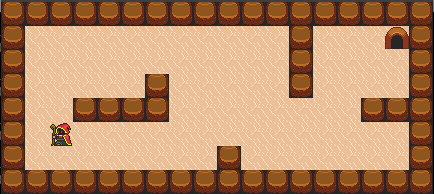
\includegraphics[width=0.5\textwidth]{./figures/experiment1}
\caption{Game environment for experiment 1}
\label{experiment1}
\end{figure}

The purpose of the first experiment is how the algorithm learns the model of the environment, or hypothesis in ILASP.
The environment are defined as a simple maze where the goal is located the right uppper corner as shown in Figure \ref{experiment1}.

The shortest path is taking the lower path instead of the upper one.

\begin{figure}[!htb]
\centering
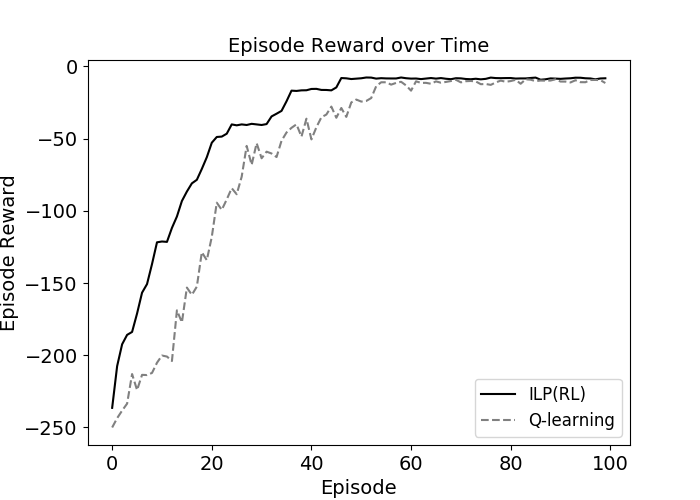
\includegraphics[width=1.0\textwidth]{./figures/experiment1_training}
\caption{Result of experiment 1 (learning curve)}
\label{experiment1_training}
\end{figure}
\begin{figure}[!htb]
\centering
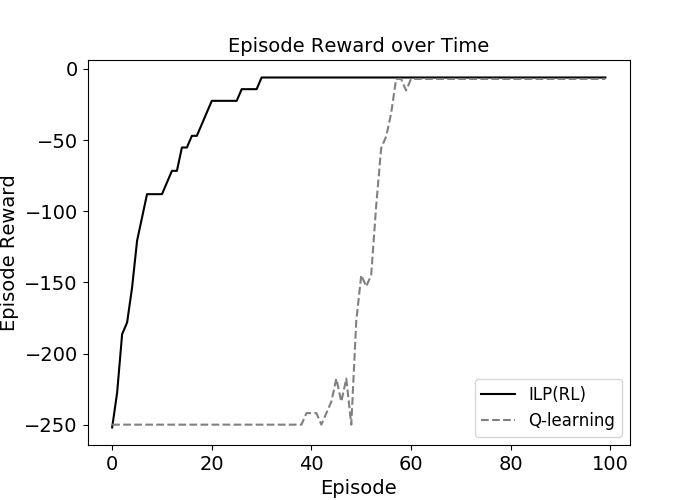
\includegraphics[width=1.0\textwidth]{./figures/experiment1_test}
\caption{Result of experiment 1 (performance)}
\label{experiment1_test}
\end{figure}

Figure \ref{experiment1_training} shows the traning performance between ILP(RL) and Q-learning.
The convergence rate of ILP(RL) is faster than Q-learning: ILP(RL) reaches the maximum reward between 40 and 50 episodes, whereas Q-learning reaches the same level at between 60 and 70 episodes.
This is because unlike Q-learning where the value function is updated with the rate of alpha, whereas ILP(RL) gradually builds the model of the environment and use the background knowledge to accurately plan.
This result is also consistent with the general notion that model-based learning (ILP(RL)) is more data-efficient than model-free learning (Q-learning).
The same trend is also shown in Figure \ref{experiment1_test}, where we measure only the performance of the policy without random exploration.

Overall this results shows that ILP(RL) converges to the optimal policy faster than benchmarks in a simple scenarios, achieving more data-efficient learning.

In addition to the data-efficient learning, what the agent has learnt with ILP(RL) is expressive.
Learnt hypotheses are shown in \ref{experiment1_hypothesis}, which is the rule of the game and easy to understand for human users.
Since the learnt hypothesis is a general concept, which can be used in a different environmet.
This transfer learning capability is also described in Experiement 3 and 4.

\begin{equation}
\begin{split}
&\textsf{state\_after(V1) :- adjacent(right, V0, V1), state\_before(V1), action(right), wall(V0).}\\
&\textsf{state\_after(V0) :- adjacent(right, V0, V1), state\_before(V0), action(left), wall(V1).}\\
&\textsf{state\_after(V1) :- adjacent(down, V0, V1), state\_before(V1), action(down), wall(V0).}\\
&\textsf{state\_after(V1) :- adjacent(up, V0, V1), state\_before(V1), action(up), wall(V0).}\\
&\textsf{state\_after(V0) :- adjacent(right, V0, V1), state\_before(V1), action(right), not wall(V0).}\\
&\textsf{state\_after(V0) :- adjacent(left, V0, V1), state\_before(V1), action(left), not wall(V0).}\\
&\textsf{state\_after(V0) :- adjacent(down, V0, V1), state\_before(V1), action(down), not wall(V0).}\\
&\textsf{state\_after(V0) :- adjacent(up, V0, V1), state\_before(V1), action(up), not wall(V0).}
\end{split}
\end{equation}
\label{experiment1_hypothesis}

In addition, we plot the learning convergence for ILASP at episode 0 in Figure \ref{experiment1_ilasp}, measured in terms of the number of hypothesis refinement to reach the final hypothesis as shown in \ref{experiment1_hypothesis}.
This shows that the agent quickly learns the hypothesis at the episode 0. The reason that the agent reaches the maximum reward at between 40 and 50 episodes, is mostly dependent on how quickly the agent finds the goal location,
which enables it to plan. Since our exploration strategy is expilon random choice, there is a promissing that a better exploration strategy further accelerates the learning process.

\begin{figure}[!htb]
\centering
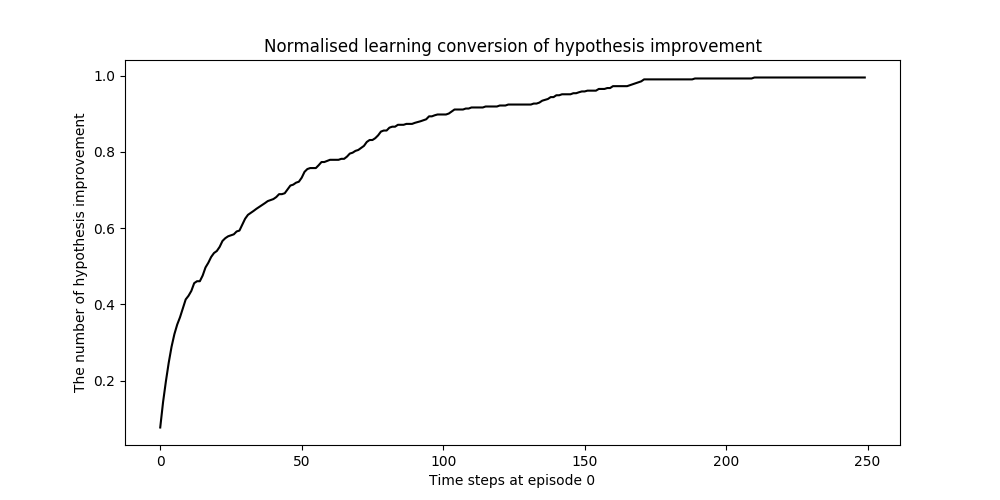
\includegraphics[width=1.0\textwidth]{./figures/experiment1_ilasp}
\caption{Normalised learning convergence by ILASP for experiment 1}
\label{experiment1_ilasp}
\end{figure}

\newpage
\subsection{Experiment Result 2}
\label{subsec:experiment_result_2}
% The game is designed such that

\begin{figure}[!htb]
\centering
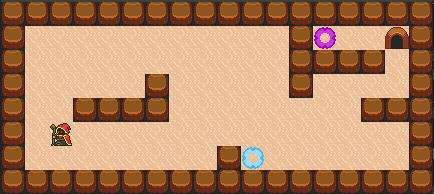
\includegraphics[width=0.5\textwidth]{./figures/experiment2}
\caption{Game environment for experiment 2}
\label{experiment3}
\end{figure}

Experiment 2 was conducted to see if the agent find a optimal path of using a teleport. In the environment shown in Figure \ref{experiment3},
there are two ways to reach the goal: using a normal path to get the goal located on the top right corner, or using a telport.
The environment is designed such that using a teleport is a shorter path and therefore gives higher total reward.
Compared to Experiment 1, two extra search spaces and concepts are added as follow:
\begin{equation*}
\begin{split}
&\textsf{\#modeb(1, link\_start(var(cell)), (positive)).}\\
&\textsf{\#modeb(1, link\_dest(var(cell)), (positive)).}
\end{split}
\end{equation*}

Where teleport links are added to the environment. The teleport link is one-way: link\_start takes the agent to link\_dest, but link\_dest does not take the agent back to link\_start.
The allows ILASP to learn additional hypothesis.
The full learning task for this experiment is in Appendix XX.

Once the agent steps onto a state where link\_start is located, it gets two positive experiences.
In this game environment, the agent moves two cells in one time step instead of one cell per time step.

Also link\_start and link\_dest need to be stored in background knowledge rather than as contex examples,
because ILASP needs to learn different hypothesis for link and non-link case.
link locations need to be available for all positive examples so that ILASP correctly learn non-link, which is shown in Figure XX below.

\begin{figure}[!htb]
\centering
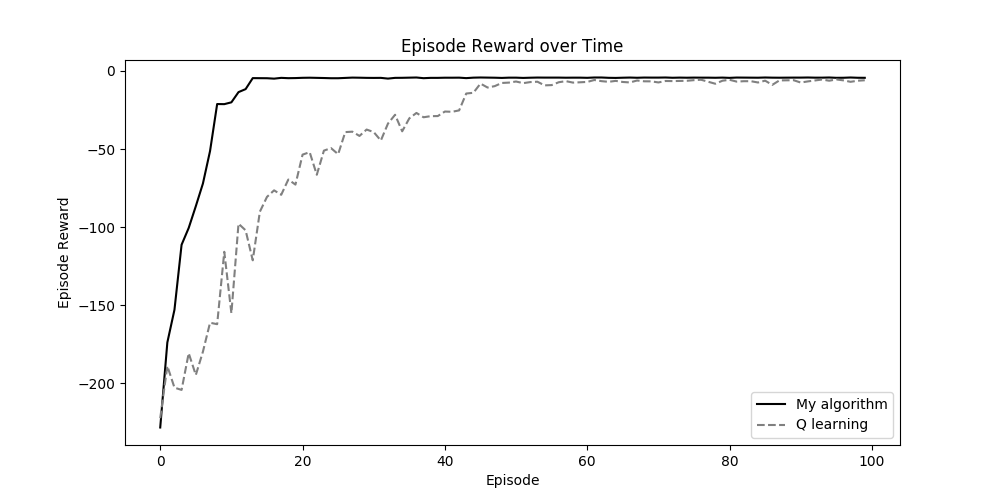
\includegraphics[width=1.0\textwidth]{./figures/experiment2_training}
\caption{Result of experiment 2 (learning curve)}
\label{experiment2_training}
\end{figure}

The training performance shown in XX, which converges faster than XX.

\begin{figure}[!htb]
\centering
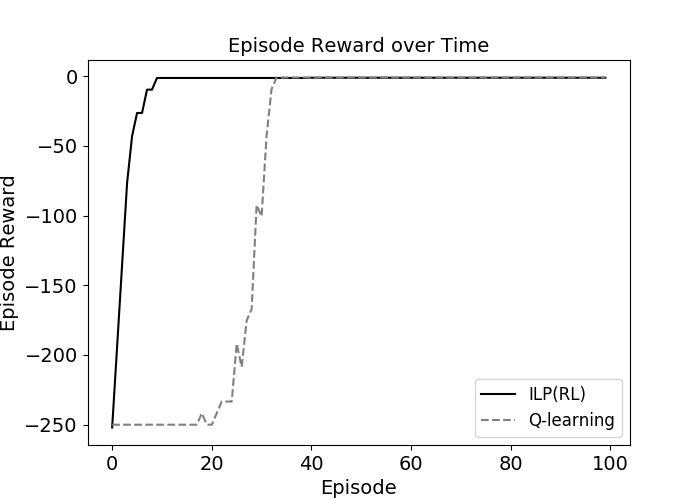
\includegraphics[width=1.0\textwidth]{./figures/experiment2_test}
\caption{Result of experiment 2 (performance)}
\label{experiment2_test}
\end{figure}

\begin{equation}
\begin{split}
&\textsf{state\_after(V1) :- link\_dest(V1).}\\
&\textsf{state\_after(V0) :- link\_dest(V0), state\_before(V0), action(right).}\\
&\textsf{state\_after(V1) :- adjacent(left, V0, V1), state\_before(V0), action(right), not wall(V1).}\\
&\textsf{state\_after(V0) :- adjacent(left, V0, V1), state\_before(V1), action(left), not wall(V0).}\\
&\textsf{state\_after(V1) :- adjacent(up, V0, V1), state\_before(V0), action(down), not wall(V1).}\\
&\textsf{state\_after(V0) :- adjacent(up, V0, V1), state\_before(V1), action(up), not wall(V0).}\\
&\textsf{state\_after(V1) :- adjacent(left, V0, V1), state\_before(V1), action(left), wall(V0).}\\
&\textsf{state\_after(V1) :- adjacent(down, V0, V1), state\_before(V1), action(down), wall(V0).}\\
&\textsf{state\_after(V1) :- adjacent(up, V0, V1), state\_before(V1), action(up), wall(V0).}
\end{split}
\label{experiment2_ilasp_imcomplete}
\end{equation}

To highlight the learning the new concept of teleport link, Figure \ref{experiment2_ilasp_imcomplete} is an intermediate incomplete hypothesis learnt by ILASP.
These hypotheses are generated just after the agent steps onto the link. However, the first hypothesis says
when link\_dest is available state\_after is true. Since link\_dest is available in background knowledge rather than context,
when solving for answer sets to generate a plan, it generates incorrect state\_after at every time step.
However, as shown in Algorithms XX, these generated state\_after are all incorrect and therefore will be added to exclusions of the next positive examples.
These exclusions will later refines hypotheses and results in Figure \ref{experiment2_ilasp_complete}, the final complete hypotheses.

Learnt hypotheses are as follow:
\begin{equation}
\begin{split}
&\textsf{state\_after(V1) :- link\_start(V0), link\_dest(V1), state\_before(V0).}\\
&\textsf{state\_after(V0) :- link\_dest(V0), state\_before(V0), action(right).}\\
&\textsf{state\_after(V1) :- adjacent(left, V0, V1), state\_before(V0), action(right), not wall(V1).}\\
&\textsf{state\_after(V0) :- adjacent(left, V0, V1), state\_before(V1), action(left), not wall(V0).}\\
&\textsf{state\_after(V1) :- adjacent(up, V0, V1), state\_before(V0), action(down), not wall(V1).}\\
&\textsf{state\_after(V0) :- adjacent(up, V0, V1), state\_before(V1), action(up), not wall(V0).}\\
&\textsf{state\_after(V1) :- adjacent(left, V0, V1), state\_before(V1), action(left), wall(V0).}\\
&\textsf{state\_after(V1) :- adjacent(down, V0, V1), state\_before(V1), action(down), wall(V0).}\\
&\textsf{state\_after(V1) :- adjacent(up, V0, V1), state\_before(V1), action(up), wall(V0).}
\end{split}
\label{experiment2_ilasp_complete}
\end{equation}

Compared the Experiment 1, there are two new hypotheses due to the presence of the teleport links.
These learnt hypotheses are also applicables to an environment where there is no link, such as a game in experiment 1.
In this case, the first two hypotheses in Figure XX are never be used since the body predicates relating to link\_start(V0), link\_dest(V1) are never be satisfied.

\begin{figure}[!htb]
\centering
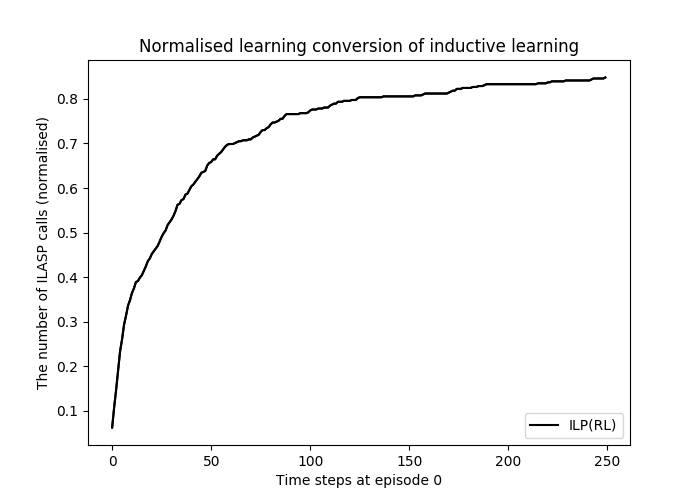
\includegraphics[width=1.0\textwidth]{./figures/experiment2_ilasp}
\caption{Normalised learning convergence by ILASP for experiment 2}
\label{experiment1_test}
\end{figure}

\newpage
\section{Transfer Learning Evaluation}
\label{sec:transfer_learning_evaluation}
\subsection{Experiment Result 3}

\begin{figure}[!htb]
\centerline{
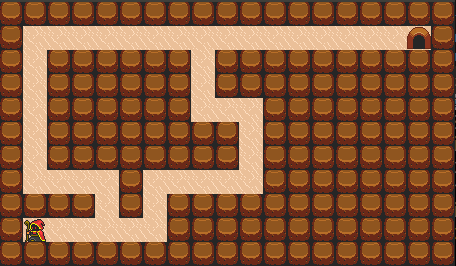
\includegraphics[width=0.5\textwidth]{./figures/experiment3_before}
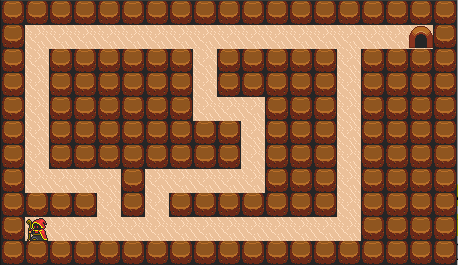
\includegraphics[width=0.5\textwidth]{./figures/experiment3_after}
}
\caption{Game environment for experiment 3: before (left) and after (right) transfer learning}
\label{experiment3}
\end{figure}

In Experiment 3, we investigated the potentials of transfer learning betweeen similar environments.
We trained the agent using the environment on the left in Figure \ref{experiment4}, and transfer the learnt hypothesis as well as positive examples to a new environment.
The learnt hypothesis is valid move of the game and a general concept that is applicable to any similar games. Positive examples are also transferred since
if there is a new concept that the agent needs to learn in a new environment, the agent needs to refine the hypothesis by running ILASP, thus the all the positice examples
are also transferred as well as hypotheses. Background knowledge are not transferred since these information are different in a new environment.
The agent starts with an empty background knowledge in the new environment and gradually collects them
as it explore the environment. The goal position is the same as in the first game and we assume that the transferred agent already knows the goal location, but the routes to the goal may be different.
While this is a limited transfer learning since the goal position is known in advance, this is still a useful transfer in cases where the rest of the environment changes.
In this experiment, we compare the two learning performance: one with transfer learning and one without it.
The result is shown in Figure \ref{experiment3_training} and \ref{experiment3_test}.

These are the hypotheses we are transferring to a new environment.
Since the complete hypothesis is already known to the agent, it can do planning from the beginning.

\begin{equation}
\begin{split}
 &\textsf{state\_after(V0) :- adjacent(right, V0, V1), state\_before(V1), action(right), not wall(V0).}\\
 &\textsf{state\_after(V0) :- adjacent(left, V0, V1), state\_before(V1), action(left), not wall(V0).}\\
 &\textsf{state\_after(V1) :- adjacent(down, V0, V1), state\_before(V0), action(up), not wall(V1).}\\
 &\textsf{state\_after(V0) :- adjacent(down, V0, V1), state\_before(V1), action(down), not wall(V0).}\\
 &\textsf{state\_after(V1) :- adjacent(right, V0, V1), state\_before(V1), action(right), wall(V0).}\\
 &\textsf{state\_after(V1) :- adjacent(left, V0, V1), state\_before(V1), action(left), wall(V0).}\\
 &\textsf{state\_after(V0) :- adjacent(up, V0, V1), state\_before(V0), action(down), wall(V1).}\\
 &\textsf{state\_after(V1) :- adjacent(up, V0, V1), state\_before(V1), action(up), wall(V0).}
\end{split}
\end{equation}

\begin{figure}[!htb]
\centering
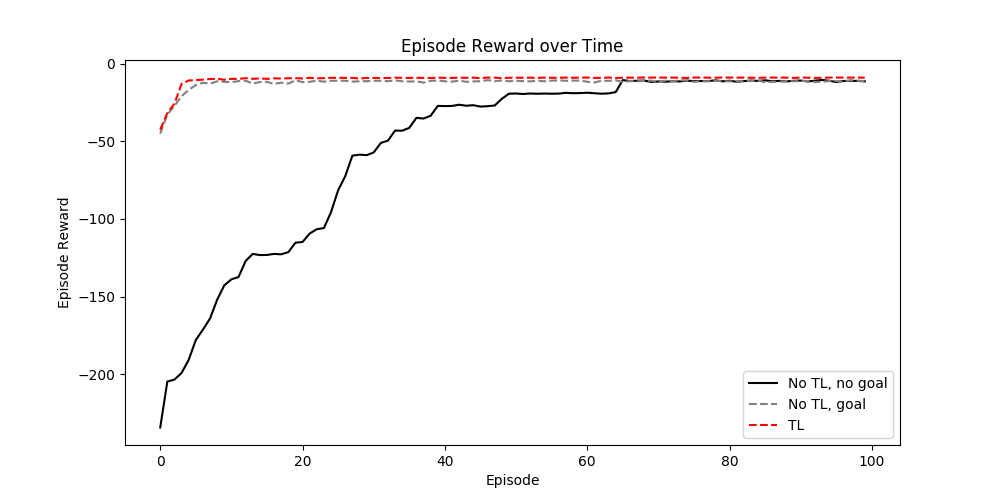
\includegraphics[width=1.0\textwidth]{./figures/experiment3_after_training}
\caption{Result of experiment 3 (learning curve)}
\label{experiment3_training}
\end{figure}

\begin{figure}[!htb]
\centering
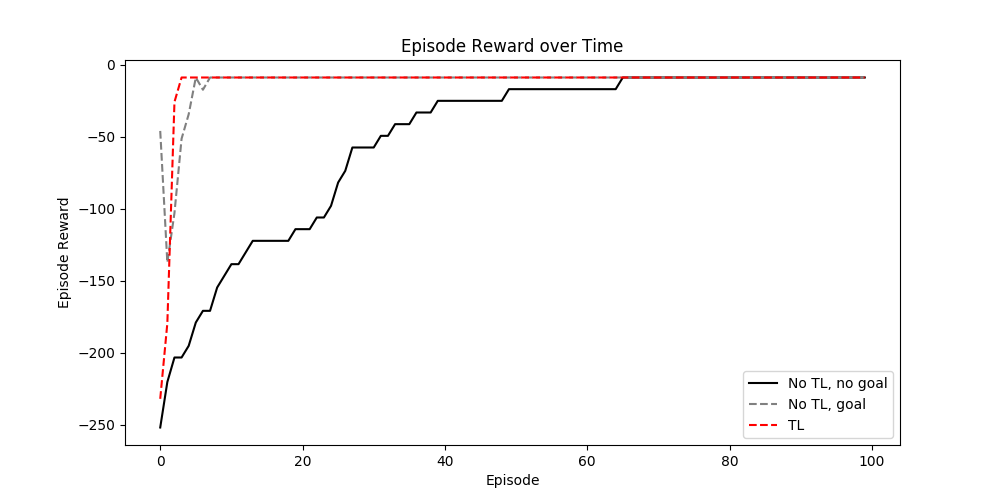
\includegraphics[width=1.0\textwidth]{./figures/experiment3_after_test}
\caption{Result of experiment 3 (performance)}
\label{experiment3_test}
\end{figure}

\subsection{Experiment Result 4}
\label{subsec:experiment_result_4}

\begin{figure}[!htb]
\centerline{
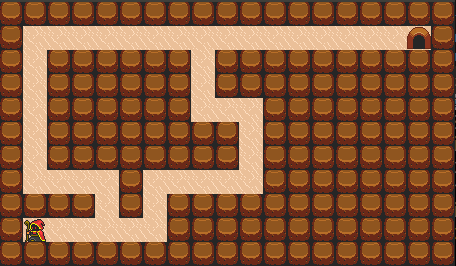
\includegraphics[width=0.5\textwidth]{./figures/experiment4_before}
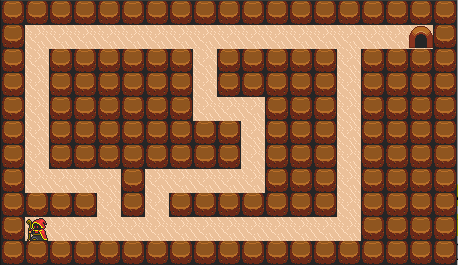
\includegraphics[width=0.5\textwidth]{./figures/experiment4_after}}
\caption{Game environment for experiment 4: before (left) and after (right) transfer learning}
\label{experiment5}
\end{figure}

Finally the hypothesis is transferred to a new environment where there is a new concept that did not exist in the first environment
and therefore the agent needs to learn it after the hypothesis is transferred.

\begin{figure}[!htb]
\centering
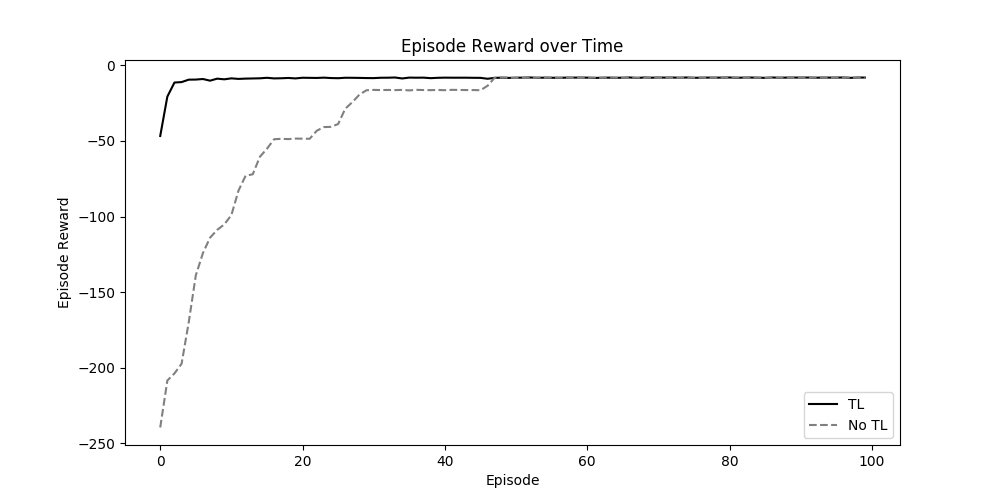
\includegraphics[width=1.0\textwidth]{./figures/experiment4_training}
\caption{Result of experiment 4 (learning curve)}
\label{experiment5_training}
\end{figure}

\begin{figure}[!htb]
\centering
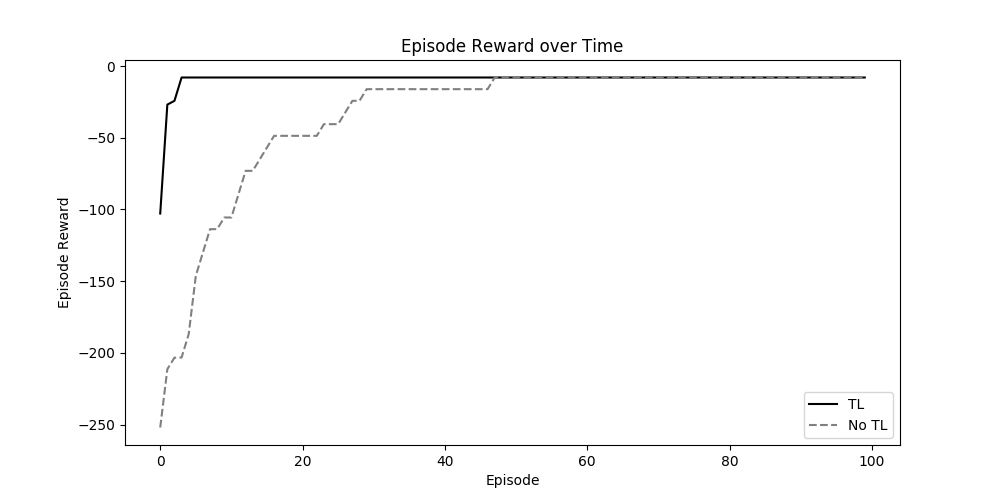
\includegraphics[width=1.0\textwidth]{./figures/experiment4_test}
\caption{Result of experiment 4 (performance)}
\label{experiment5_test}
\end{figure}

\begin{equation}
\begin{split}
&\textsf{state\_after(V1) :- link\_start(V0), link\_dest(V1), state\_before(V0).}\\
&\textsf{state\_after(V1) :- adjacent(left, V0, V1), state\_before(V0), action(right), not wall(V1).}\\
&\textsf{state\_after(V0) :- adjacent(left, V0, V1), state\_before(V1), action(left), not wall(V0).}\\
&\textsf{state\_after(V1) :- adjacent(up, V0, V1), state\_before(V0), action(down), not wall(V1).}\\
&\textsf{state\_after(V0) :- adjacent(up, V0, V1), state\_before(V1), action(up), not wall(V0).}\\
&\textsf{state\_after(V0) :- adjacent(left, V0, V1), state\_before(V0), action(right), wall(V1).}\\
&\textsf{state\_after(V1) :- adjacent(left, V0, V1), state\_before(V1), action(left), wall(V0).}\\
&\textsf{state\_after(V0) :- adjacent(up, V0, V1), state\_before(V0), action(down), wall(V1).}\\
&\textsf{state\_after(V1) :- adjacent(up, V0, V1), state\_before(V1), action(up), wall(V0).}
\end{split}
\label{experiment4_ilasp}
\end{equation}

% In simple environments, we show that the agent learns rule of the game faster than existing RL algorithms, learnt concepts is easy to understand for human users.
% We also show that the learnt hypothesis is a general concept and can be applied to other environment to mitigate learning process.

% The full hypotheses were learnt in the very early phase of learning and exploration phase. Thus with sufficient exploration, the model of the environment is correct
% and therefore it is able to find the optimal policy/path. 

% We show that ILP(RL) is able to solve a reduced MDP where the rewards are assumed to be associated with a sequence of actions planned as answer sets.
% Although this is a limitated solution, there is a potential to expand it to solve full MDP as discussed in Further Research. 

% TODO more details on the strength of the algorithm. 
% Validity

\section{Discussion}

Although this is the first time and inductive logic programming is applied into reinforcement leaning and there are new interesting property for ILP(RL),
there are two major limitations with the current framework.

\subsection{Scalability}
The first limitation is scalability. As pointed in XXX or XXX,
ILP framework is known to be less scalable. The current framework is tested in a relatively simple environments, 
and proven to be work better than RL algorithsm in terms of the number of episodes that is needed to converge to an optimal policy.
However, learning in each episode is relatively slower than that of RL. 
This is shown in XXX, which shows average learnint time for ILASP. 

This limitation is theoretically discussed in XXX, where the complexity of deciding satisfiability is 
$\sum_{2}^{P}$-complete. Since there is no negative examples used in our current framework, the complexity is NP-complete.

Whereas Q-learning update value function in the same way whether there is a new concept such as teleport links.

Figure XXX shows traning times for Experiment 1 and 2.

ILASP learning time for Experiment 1 and 2. 

Unlike existing reinforcement learning,
out algorithm refines hypothesis at every time steps within the same episode.
Thus even though the efficiency in terms of the number of iteration is higher,
training time within each iteration tends to be lower.

\subsection{Flexibility}
While most of existing reinforcement learning works in different kinds of environment without pre-configuration, our algorithm
needs to define search space for learning hypothesis. As explained in the experiment 3, it was necessary to add two extra modeb before training.
Thus the algorithm may not be feasible in cases where these learning concepts were unknown or difficult to define. 
In addition, not only it needs search space, surrounding information is assumed to be known to the agent. 
While this assumption may be reasonable in many cases, this is not common in traditional reinforcement learning setting.

The current framework does not make use of rewards the agent collects and mainly uses the location of the goal for planning.
In some senarios, there may not be a termination state (goal) and instead there may be a different purpose to gain these rewards. 
Since the current implementation is dependent on finding the goal for planning rather than maximing total rewards, which is the common objective for most of RL algorithms,
the application of the current framework may be limited to particular types of problems.

Another question remains to how to extend the framework to more realistic senarios. RL works in more complex environments such as 3D or real physical environment, 
whereas the experiences of the agent in the current framework need to be expressed as ASP syntax, thus expressing continuous states rather than discrete states is challenging.



\chapter{Related Work}
\label{related_work}
In this section, I summarise recent studies related to symbolic (deep) reinforcement learning.

 \cite{Garnelo2016} introduced Deep Symbolic Reinforcement Learning (DSRL), a proof of concept for incorporating symbolic front end as a means of converting low-dimensional symbolic representation into spatio-temporal representations, which will be the state transitions input of reinforcement learning. DSRL extracts features using convolutional neural newtworks (CNNs) \cite{LeCunL1998} and an autoencoder, which are transformed into symbolic representations for relevant object types and positions of the objects. These symbolic representations represent abstract state-space, which are the inputs for the Q-learning algorithm to learn a policy on this particular state-space. DSRL was shown to outperform DRL in stochastic variant environments.
However, there are a number of drawbacks to this approach. First, the extraction of the individual objects was done by manually defined threhold of feature activation values, given that the games were geometrically simple. Thus this approach would not scale in geometrically complex games. Second, using deep neural network front-end might also cause a problem. As demonstrated in \cite{Su2017}, a single irrelevant pixel could dramatically influence the state through the change in CNNs.
In addition, while proposed method successfully used symbolic representations to achieve more data-efficient learning, there is still the potential to apply symbolic learning to those symbolic representations to further improve the learning efficiency, which is what we attemp to do in this paper.
\cite{Garcez2018} further explored this symbolic abstraction approach by incorporating the relative position of each object with respect to every other object rather than absolute object position. They also assign priority to each Q-value function based on the relative distance of objects from an agent.

\cite{Zambaldi2018} added relational reinforcement learning, a classical subfield of research aiming to combining reinforcement learning with relational learning or Inductive Logic Programming,  which added more abstract planning on top of DSRL approach. The new mode was then applied to much more complicate game environment than that used by \cite{Garnelo2016}.
%They incorporated a deep RL with architectural inductive biases
%structured representations of the game, and relatioal reasoning.
%The use of symbolic representations to achieve data-efficient learning was traditionally discussed in relational reinforcement learnign (RLL).
This idea of adding planning capability align with our approach of using ILP to improve a RL agent. We explore how to effectively learn the model of the environment and effectively use it to facilitate data-efficient learning and transfer learning capability.

%Transparency and interpretable capability of the model is another important aspect for machine learning applications.

%The history of data-efficient learning

Another approach for using symbolic reinforcement learning is storing heuristics expressed by knowledge bases [\cite{Apeldoorn2017}).  An agent lerans the concept of \textit{Hierarchical Knowledge Bases (HKBs)} (which is defined in more details in \cite{Apeldoorn2016} and \cite{Apeldoorn}] at every iteration of training, which contain multiple rules (state-action pairs).  The agent then is able to decide itself when it should exploit the heuristic rather than the state-action pairs of the RL using  \textit{Strategic Depth}. This approach effectively uses the heuristic knowledge bases, which acts as a sym-symbolic model of the game.

Another field related to our research is the combining of ASP and RL. The original concept of combining ASP and RL was in \cite{Ferreira2017}, where they developed an algorithm that efficiently finds the optimal solution of an MDP of non-stationary domains by using ASP to find the possible trajectories of an MDP. This approach focused more on efficient update of the Q function rather than inductive learning. In order to find stationary sets, an extension of ASP called BC\textsuperscript{+}, an action language,  was used. BC\textsuperscript{+} can directly translate the agent's actions into ASP form, and provide sequences of actions in answer sets.

%ASP BC\textsuperscript{+} translation was done manually.

%Incorporation of logic into reinforcement learning dates back to the study of relational reinforcement learning,

%There are a number of research conducted in applying DNN to symbolic reasoning.
%[From GamePlay to Symbolic Reasoning]



\chapter{Discussion}
\label{discussion}
\section{Strengths}
\label{strengths}

To my knowledge, this is the first attemp that inductive logic programming is incorporated into a reinforcement learning senario to facilitate learning process.
In simple environments, we show that the agent learns rule of the game faster than existing RL algorithms, learnt concepts is easy to understand for human users.
We also show that the learnt hypothesis is a general concept and can be applied to other environment to mitigate learnig process.

The full hypotheses were learnt in the very early phase of learning and exploration phase. Thus with sufficient exploration, the model of the environment is correct
and therefore it is able to find the optimal policy/path. 

We show that ILP(RL) is able to solve a reduced MDP where the rewards are assumed to be associated with a sequence of actions planned as answer sets.
Although this is a limitated solution, there is a potential to expand it to solve full MDP as discussed in Further Research. 

TODO more details on the strength of the algorithm. 
Validity

\section{Limitations}

Although this is the first time and inductive logic programming is applied into reinforcement leaning and there are new interesting property for ILP(RL),
there are two major limitations with the current framework.

\subsection{Scalability}
The first limitation is scalability. As pointed in XXX or XXX,
ILP framework is known to be less scalable. The current framework is tested in a relatively simple environments, 
and proven to be work better than RL algorithsm in terms of the number of episodes that is needed to converge to an optimal policy.
However, learning in each episode is relatively slower than that of RL. 
This is shown in XXX, which shows average learnint time for ILASP. 

This limitation is theoretically discussed in XXX, where the complexity of deciding satisfiability is 
$\sum_{2}^{P}$-complete. Since there is no negative examples used in our current framework, the complexity is NP-complete.

Whereas Q-learning update value function in the same way whether there is a new concept such as teleport links.

Figure XXX shows traning times for Experiment 1 and 2.

ILASP learning time for Experiment 1 and 2. 

Unlike existing reinforcement learning,
out algorithm refines hypothesis at every time steps within the same episode.
Thus even though the efficiency in terms of the number of iteration is higher,
training time within each iteration tends to be lower.

\subsection{Flexibility}
While most of existing reinforcement learning works in different kinds of environment without pre-configuration, our algorithm
needs to define search space for learning hypothesis. As explained in the experiment 3, it was necessary to add two extra modeb before training.
Thus the algorithm may not be feasible in cases where these learning concepts were unknown or difficult to define. 
In addition, not only it needs search space, surrounding information is assumed to be known to the agent. 
While this assumption may be reasonable in many cases, this is not common in traditional reinforcement learnig setting.

The current framework does not make use of rewards the agent collects and mainly uses the location of the goal for planning.
In some senarios, there may not be a termination state (goal) and instead there may be a different purpose to gain these rewards. 
Since the current implementation is dependent on finding the goal for planning rather than maximing total rewards, which is the common objective for most of RL algorithms,
the application of the current framework may be limited to particular types of problems.

Another question remains to how to extend the framework to more realistic senarios. RL works in more complex environments such as 3D or real physical environment, 
whereas the experiences of the agent in the current framework need to be expressed as ASP syntax, thus expressing continuous states rather than discrete states is challenging.

\section{Further Research}
\label{further_research}

Having stated the limitations of the current framework, we discuss some of the possible improments and further research in this section.

This is a proof of concept, a new type of model-based reinforcement learning using inductive logic programming. 

More complicated environment

More general transfer learning.

Only empirically correct, no theoreticaly guarantee

Dynamic environment like moving enermy etc.

Non-stationality possible to be handled??

Our approach is similar to experience replay ??

More promissing approach is to combine RL algorithm and using ILP approach to complement each other, rather than replacing the bellman equation altogether. 

\subsection{Value Iteration Approach}

The proposed architecture is not finalised and will be reviewed regularly as we do more research.
More research needs to be devoted to finalising the overall architecture, and the following issues in particular need to be considered.

\subsection{Weak Constraint}

\begin{itemize}

\item Further investigation of whether ILASP can learn the concept of adjacent, which is crucial concept to know in any environment.
\item How to generalise the agent's model when the environment changes. The new environment could be very similar to the previous one, or could be a completely different environment thus the agent should create a new internal model rather than generalising the existing model.
\item The current proposed architecture is based on Dyna with simulated experiences. However, this might not be the best overall architecture, and the feasibility of using simulated experience with the learnt model with ILASP needs to be further investigated.

\item Possibility of using other representational concepts such as \textit{Predictive Representations of State} or \textit{Affordance} \cite{Sridharan2017} for the agent's learning task. These concept have not been considered at the moment, but could help better transfer learning.

\item Preparation for a backup plan in case ILASP approach does not work, so that the researchs feasible within 3 months of the researcheriod.

\end{itemize}

\subsection{Generalisation of the Current Approach}

Learning the concept of being adjacent

\chapter{Conclusion}
\label{conclusion}


\section{Contribution}
\label{contribution}

 To my knowledge, this is the first time that both symbolic learning method is incorporated into a reinforcement learning to facilitate learning process


\section{Conclusion}
\label{conclusion}


\clearpage
\appendix
\pagebreak
\begin{appendices}

To our best knowledge, there is no particular ethical considerations for this particular research listed in Table \ref{table:ethics_checklist}. 
Although this project is part of artificial intelligence in both inductive logic programming as well as reinforcement learning, it is a preliminary research and all the experiments were conducted using a game environment. Therefore there is no concerns for misuse or real applications.
{
\renewcommand*{\arraystretch}{1.3}
\begin{longtable}{ |p{13.2cm}|p{0.6cm}|p{0.6cm}| }
\label{table:ethics_checklist}
\hline
 & \bf Yes & \bf No \\
\hline

\multicolumn{3}{|l|}{\cellcolor{green!25}\bf Section 1: HUMAN EMBRYOS/FOETUSES} \\
\hline

Does your project involve Human Embryonic Stem Cells? & & \checkmark\\
\hline

Does your project involve the use of human embryos? & & \checkmark\\
\hline

Does your project involve the use of human foetal tissues / cells? & & \checkmark\\
\hline

\multicolumn{3}{|l|}{\cellcolor{green!25}\bf Section 2: HUMANS} \\
\hline

Does your project involve human participants? & & \checkmark\\
\hline

\multicolumn{3}{|l|}{\cellcolor{green!25}\bf Section 3: HUMAN CELLS / TISSUES} \\
\hline

Does your project involve human cells or tissues? (Other than from “Human Embryos/Foetuses” i.e. Section 1)? & & \checkmark\\
\hline

\multicolumn{3}{|l|}{\cellcolor{green!25}\bf Section 4: PROTECTION OF PERSONAL DATA} \\
\hline

Does your project involve personal data collection and/or processing? & & \checkmark\\
\hline

Does it involve the collection and/or processing of sensitive personal data (e.g. health, sexual lifestyle, ethnicity, political opinion, religious or philosophical conviction)? & & \checkmark\\
\hline

Does it involve processing of genetic information? & & \checkmark\\
\hline

Does it involve tracking or observation of participants? It should be noted that this issue is not limited to surveillance or localization data. It also applies to Wan data such as IP address, MACs, cookies etc. & & \checkmark\\
\hline

Does your project involve further processing of previously collected personal data (secondary use)? For example Does your project involve merging existing data sets? & & \checkmark\\
\hline

\multicolumn{3}{|l|}{\cellcolor{green!25}\bf Section 5: ANIMALS} \\
\hline

Does your project involve animals? & & \checkmark\\
\hline


\multicolumn{3}{|l|}{\cellcolor{green!25}\bf Section 6: DEVELOPING COUNTRIES} \\
\hline

Does your project involve developing countries? & & \checkmark\\
\hline

If your project involves low and/or lower-middle income countries, are any benefit-sharing actions planned? & & \checkmark\\
\hline

Could the situation in the country put the individuals taking part in the project at risk? & & \checkmark\\
\hline

\multicolumn{3}{|l|}{\cellcolor{green!25}\bf Section 7: ENVIRONMENTAL PROTECTION AND SAFETY} \\
\hline

Does your project involve the use of elements that may cause harm to the environment, animals or plants? & & \checkmark\\
\hline

Does your project deal with endangered fauna and/or flora /protected areas? & & \checkmark \\
\hline

Does your project involve the use of elements that may cause harm to humans, including project staff? & & \checkmark\\
\hline

Does your project involve other harmful materials or equipment, e.g. high-powered laser systems? & & \checkmark\\
\hline


\multicolumn{3}{|l|}{\cellcolor{green!25}\bf Section 8: DUAL USE} \\
\hline

Does your project have the potential for military applications? & & \checkmark\\
\hline

Does your project have an exclusive civilian application focus? & & \checkmark\\
\hline

Will your project use or produce goods or information that will require export licenses in accordance with legislation on dual use items? & & \checkmark\\
\hline

Does your project affect current standards in military ethics – e.g., global ban on weapons of mass destruction, issues of proportionality, discrimination of combatants and accountability in drone and autonomous robotics developments, incendiary or laser weapons? & & \checkmark\\
\hline

\multicolumn{3}{|l|}{\cellcolor{green!25}\bf Section 9: MISUSE} \\
\hline

Does your project have the potential for malevolent/criminal/terrorist abuse? & & \checkmark\\
\hline

Does your project involve information on/or the use of biological-, chemical-, nuclear/radiological-security sensitive materials and explosives, and means of their delivery? & & \checkmark\\
\hline

Does your project involve the development of technologies or the creation of information that could have severe negative impacts on human rights standards (e.g. privacy, stigmatization, discrimination), if misapplied? & & \checkmark \\
\hline

Does your project have the potential for terrorist or criminal abuse e.g. infrastructural vulnerability studies, cybersecurity related project? & & \checkmark\\
\hline

\multicolumn{3}{|l|}{\cellcolor{green!25}\bf Section 10: LEGAL ISSUES} \\
\hline

Will your project use or produce software for which there are copyright licensing implications? & & \checkmark \\
\hline

Will your project use or produce goods or information for which there are data protection, or other legal implications? & & \checkmark\\
\hline

\multicolumn{3}{|l|}{\cellcolor{green!25}\bf Section 11: OTHER ETHICS ISSUES} \\
\hline

Are there any other ethics issues that should be taken into consideration? & & \checkmark \\
\hline

\caption{Ethics Checklist}
\label{ethics_table}
\end{longtable}

}




This is the full learning task for ILASP in the experiment 1. 

\begin{flalign*}
    &\textsf{state\_after(V1) :- link\_dest(V1).}&\\
    &\textsf{cell((0..7, 0..6)).}&\\
    &\textsf{adjacent(right, (X+1,Y),(X,Y)):- cell((X,Y)), cell((X+1,Y)).}&\\
    &\textsf{adjacent(left,(X,Y),  (X+1,Y)) :- cell((X,Y)), cell((X+1,Y)).}&\\
    &\textsf{adjacent(down, (X,Y+1),(X,Y))   :- cell((X,Y)), cell((X,Y+1)).}&\\
    &\textsf{adjacent(up,   (X,Y),  (X,Y+1)) :- cell((X,Y)), cell((X,Y+1)).}&\\
    &\textsf{\#modeh(state\_after(var(cell))).}&\\
    &\textsf{\#modeb(1, adjacent(const(action), var(cell), var(cell))).}&\\
    &\textsf{\#modeb(1, state\_before(var(cell)), (positive)).}&\\
    &\textsf{\#modeb(1, action(const(action)),(positive)).}&\\
    &\textsf{\#modeb(1, wall(var(cell))).}&\\
    &\textsf{\#max\_penalty(50).}&\\
    &\textsf{\#constant(action, right).}&\\
    &\textsf{\#constant(action, left).}&\\
    &\textsf{\#constant(action, down).}&\\
    &\textsf{\#constant(action, up).}&
\end{flalign*}
\label{appendix:learning_task}

% \#pos({state\_after((1,4))}, {state\_after((2,4)),state\_after((1,5)),state\_after((0,4)),state\_after((1,3))}, {state\_before((1,4)). action(non). wall((1, 5)). wall((0, 4)). }).
% \#pos({state\_after((1,3))}, {state\_after((2,4)),state\_after((1,5)),state\_after((0,4)),state\_after((1,4))}, {state\_before((1,4)). action(up). wall((1, 5)). wall((0, 4)). }).
% \#pos({state\_after((1,3))}, {state\_after((2,3)),state\_after((1,4)),state\_after((0,3)),state\_after((1,2))}, {state\_before((1,3)). action(right). wall((2, 3)). wall((0, 3)). }).
% \#pos({state\_after((1,3))}, {state\_after((2,3)),state\_after((1,4)),state\_after((0,3)),state\_after((1,2))}, {state\_before((1,3)). action(right). wall((2, 3)). wall((0, 3)). }).
% \#pos({state\_after((1,3))}, {state\_after((2,3)),state\_after((1,4)),state\_after((0,3)),state\_after((1,2))}, {state\_before((1,3)). action(right). wall((2, 3)). wall((0, 3)). }).
% \#pos({state\_after((1,4))}, {state\_after((2,3)),state\_after((0,3)),state\_after((1,2)),state\_after((1,3))}, {state\_before((1,3)). action(down). wall((2, 3)). wall((0, 3)). }).
% \#pos({state\_after((2,4))}, {state\_after((1,5)),state\_after((0,4)),state\_after((1,3)),state\_after((1,4))}, {state\_before((1,4)). action(right). wall((1, 5)). wall((0, 4)). }).
% \#pos({state\_after((1,4))}, {state\_after((3,4)),state\_after((2,5)),state\_after((2,3)),state\_after((2,4))}, {state\_before((2,4)). action(left). wall((2, 5)). wall((2, 3)). }).
This is the full learning task for ILASP in the experiment 1. 
The syntax and time are added for planning purpose. 

\lstinputlisting[
  caption  = {ASP program for Experiment 1},
]{appendix_asp.pl}

\end{appendices}




%% bibliography
\bibliography{references}
\bibliographystyle{ieeetr}

\end{document}
